%%%%%%%%%%%%%%%%%%%%%%%%%%%%%%%%%%%%%%%%%%%%%%%%%%%%%%%%%%%%%%%%%%% 
%                                                                 %
%                            CHAPTER TWO                          %
%                                                                 %
%%%%%%%%%%%%%%%%%%%%%%%%%%%%%%%%%%%%%%%%%%%%%%%%%%%%%%%%%%%%%%%%%%% 
 
\chapter{Hydration of Clay Minerals}
\section{Historical Approaches}
The tendency of montmorillonite clays (and other similar phylosilicate clay minerals) to swell when in the presence of water has previously been well investigated. In order to study this hydration mechanism, many different experimental methods have been devised over the years. Some of these are quite intricate, requiring specialized equipment in order to conduct such experiments, while others were much simpler. Briefly described here are two of the methods which are more widely accepted.

First is the method of water vapor adsorption. To achieve a greater control over this technique, Aldrich, Hellman, and Jackson developed a humidifier with the specific intent of being able to use it throughout conducting XRD measurements \cite{aldrich1944hydration}. Maintaining a relative humidity of approximately $p/p_0=0.92$, the samples were able to remain in a stable environment throughout the experiment. Such mechanisms have become quite standard in more recent years. Brahim, Armagan, Besson, and Tchoubar invented a chamber which could be mounted on the X-ray diffractometer, and contain the sample in a similar manner \cite{brahim1986methode}. XRD is often used to measure the basal spacing between clay sheets, using the relationship provided by Braggs law:
\begin{equation}
	\lambda = 2d\sin(\theta)
\end{equation}
where $\lambda$ is the wavelength of the incident X-ray, $d$ is the distance between sheets, and $\theta$ is the angle between the clay sheet surface, and the incident beam. Devices of similar function have been used in many other papers as well. The downfall of such a device is its complexity and cost to build. It must be ensured that it can be properly mounted with the diffractometer, and then there is the issue of creating an air supply with a bubbler and then regulating this humidity.

Another method to study the hydration of smectites is thermogravimetric analysis. Here, a sample is placed in a small furnace, where it also sits upon a highly sensitive microbalance. As the samples are heated, water on the clay surface, as well as the intercalated water begin to evaporate and leave the clay. This of course changes its mass which is measured by the balance. Such a methodology was used by Bishop, Pieters, and Edwards \cite{bishop1994infrared}. Of course, the obvious hindrance of such a method is the fact that it is unidirectional. Once heated, the air containing the moisture is vacated from the devices, and usually temperatures of over 900$^\circ$C are obtained, which denatures the clay such as in Bérend et. al. \cite{berend1995mechanism}. Due to the temperatures involved and the insulation required, it is not possible to conduct any other measurements at the same time, such as shown with the previously mentioned devices.

Combinations of these two methods have also been used as well, such as by Johnston, Sposito, and Erickson. In their paper, a special chamber is used to maintain humidity and also allow for infrared spectroscopic measurements, similar to the chambers made for XRD. The described device also has a microbalance which is able to measure changes in the sample mass at the same time. All of these methods however are either complicated to implement and build, expensive, or both. This has prompted the search for an alternative method of controlling the hydration of montmorillonite samples in a controlled fashion which is less costly and easy to implement.

\section{Method of Saturated Salt Solutions}
One such method which could possibly meet the above criteria are saturated salt solutions. Varying salts, mixed with water to the point of saturation, maintain specific relative humidities, depending on the exact salt utilized \cite{young1967humidity}. In this portion of the presented research, three different salts were used in an attempt to maintain a relative humidity necessary to facilitate the formation of a bilayer or trilayer of intercalated water in Li montmorillonite samples. Li exchanged clay was used, as it is the easiest to hydrate, due to the small size of the cation \cite{mering1964gonflement}.

\subsection{Experimental Methods}

\subsubsection{Preparation of Saturated Salt Solutions}
Salts were mixed in with distilled water in a large plastic vial until sediment began to accumulate at the base of the vial, guaranteeing complete saturation. These solutions were then poured into the base of plastic desiccators. The salts used were $(NH_4)_2SO_4$, $KNO_3$, and $K_2SO_4$. These three were chosen as they have been shown to maintain humidities of $p/p_0=0.8$, $p/p_0=0.92$, and $p/p_0=0.97$ respectively at room temperature \cite{wexler1954relative}. These humidities were chosen as it had previously been shown that only relative humidities of $p/p_0=0.9$ or greater are able to produce a homogeneous bilayer in clay samples \cite{berend1995mechanism}, \cite{mering1946hydration}. Little precision is needed in this portion of the experiment, as long as it is ensured that the solutions are indeed saturated, and no more salt my be absorbed by the water.

\subsubsection{Preparation of Clay Samples}
The same Li exchanged montmorillonite was used to produce two different types of samples: powder and disks. Typically, clay powder is used for experiments which involve hydration of the sample \cite{aldrich1944hydration}, \cite{berend1995mechanism}, \cite{johnston1992vibrational}. The clay powder was placed on sheets of weigh paper, which were in turn placed inside of desiccators where the saturated salt solutions were present. The samples would then remain there for varying amounts of time until XRD measurements were conducted on them.

\begin{figure}
	\centering
	\begin{subfigure}{.5\textwidth}
		\centering
		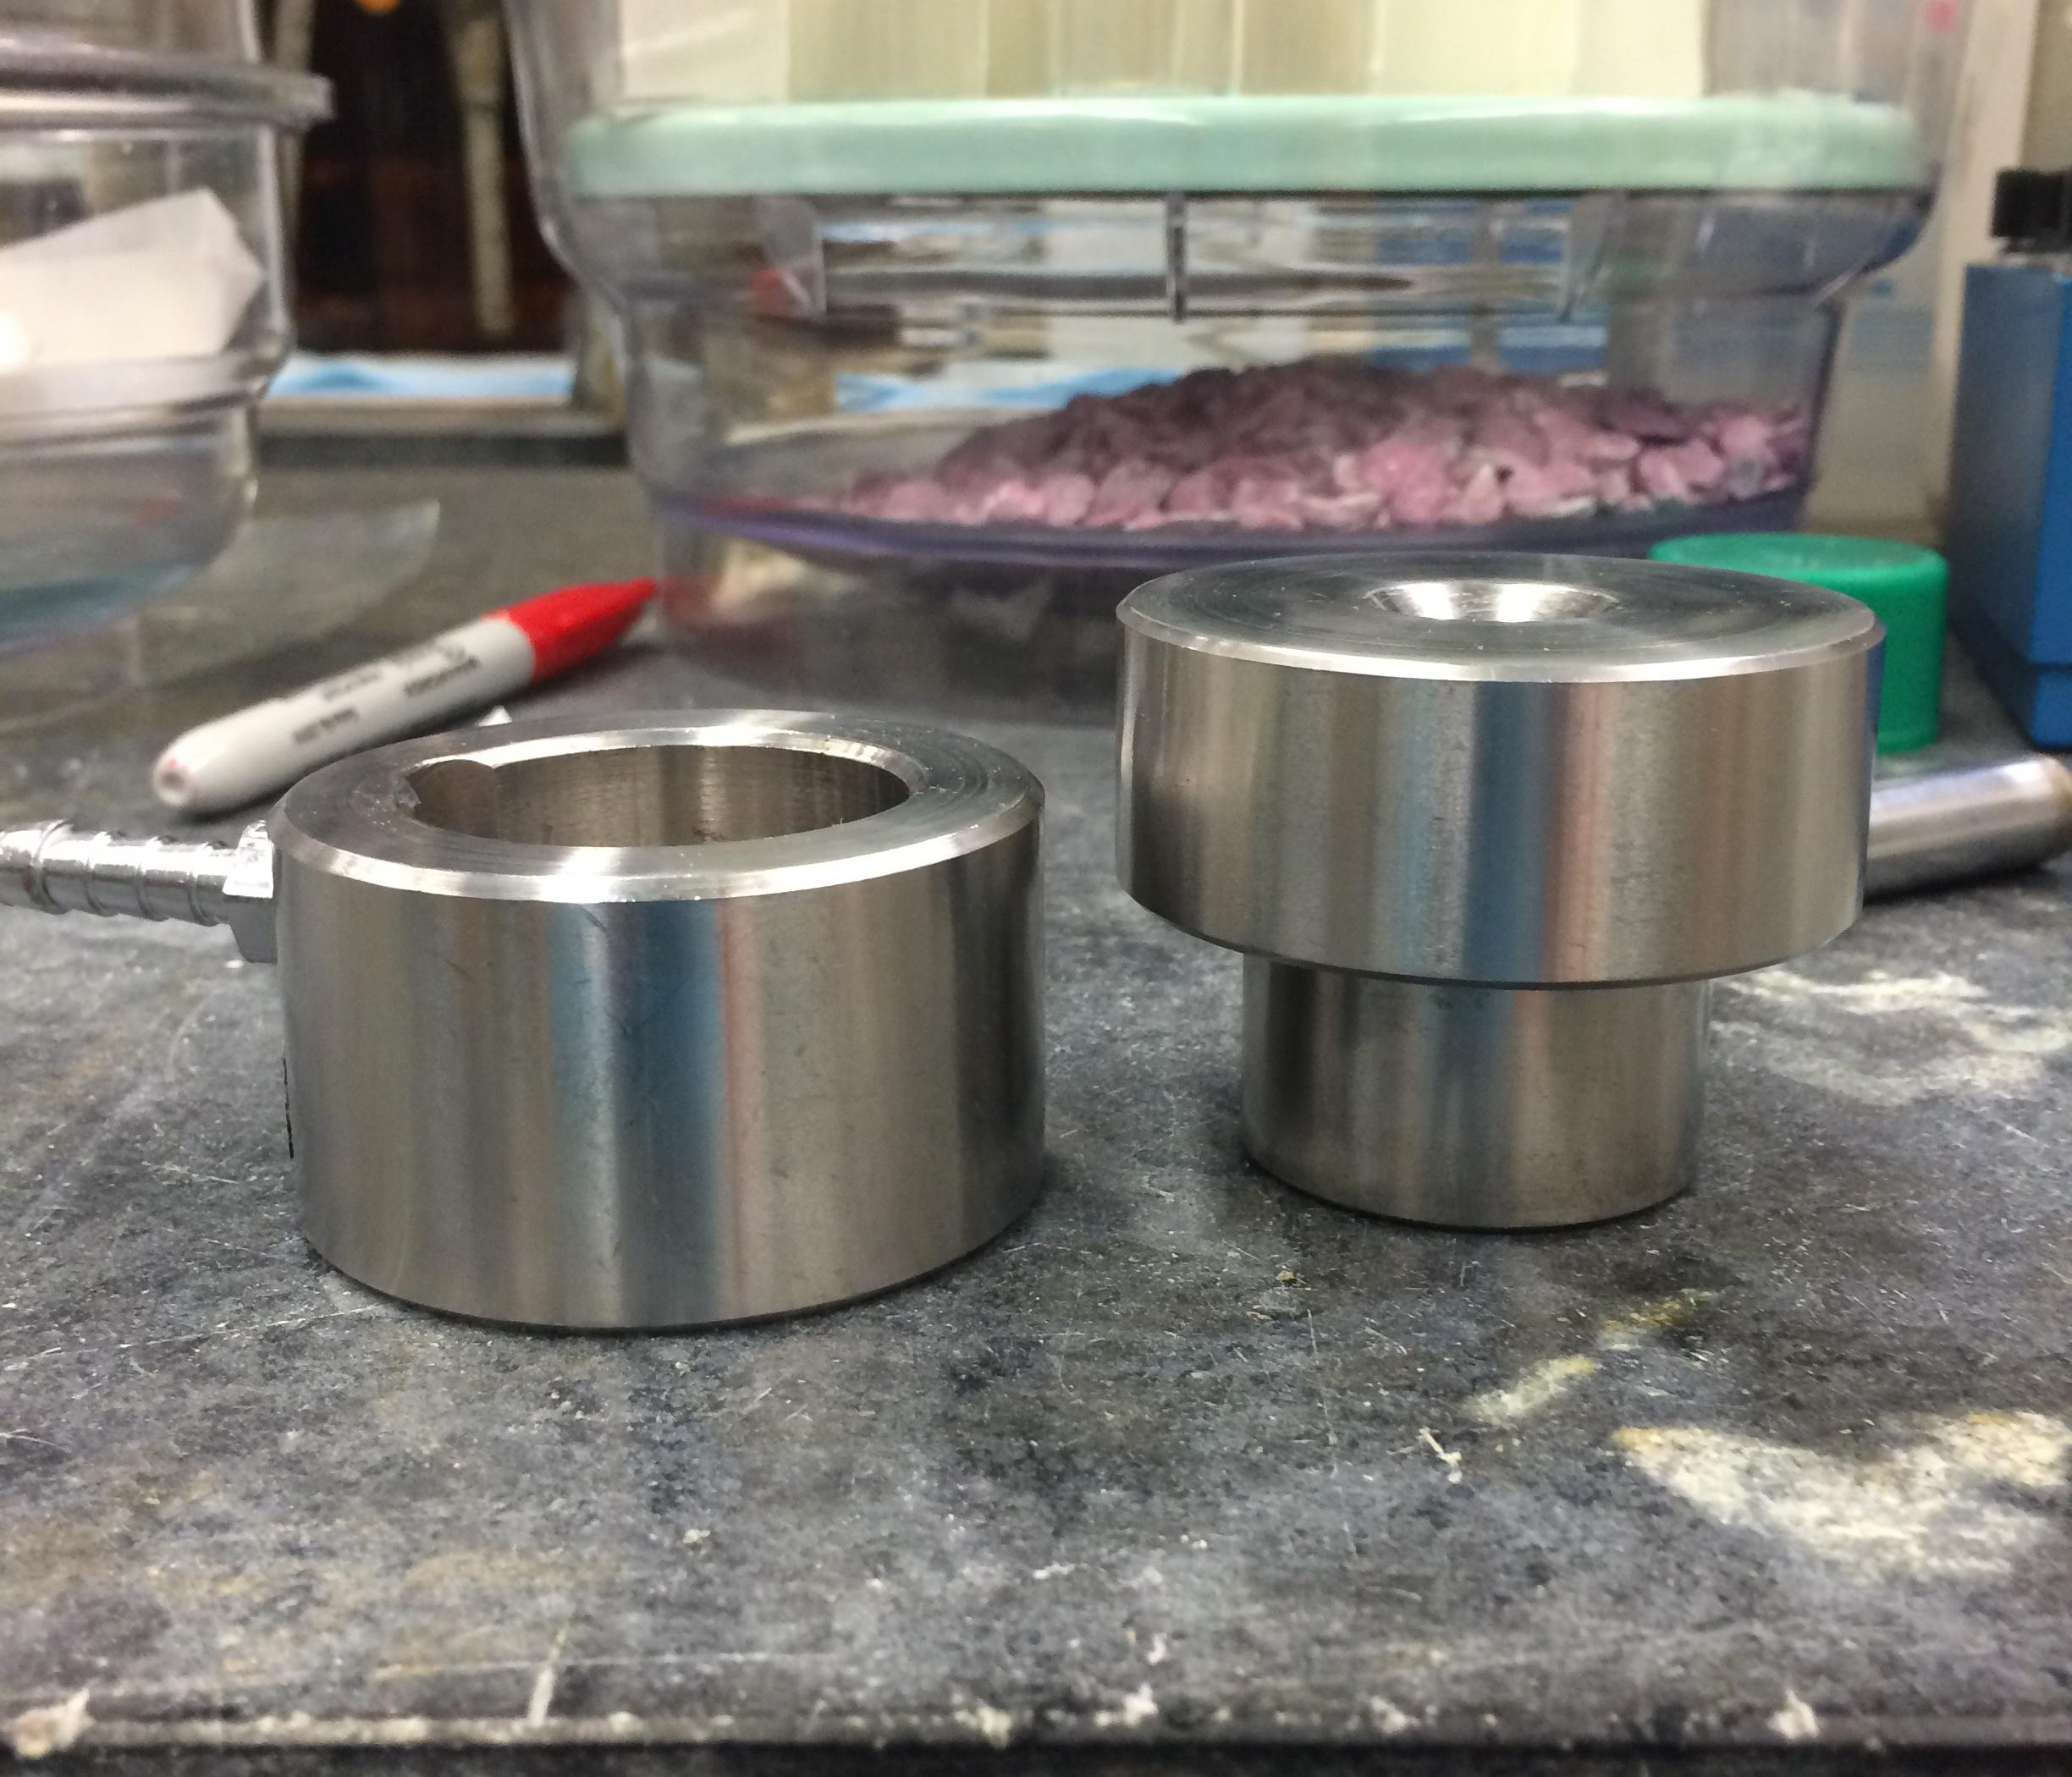
\includegraphics[scale=0.12]{images/die_opened.jpg}
		\caption{The two halves of the KBr die separated.}
		\label{fig:die_opened}
	\end{subfigure}%
	\begin{subfigure}{.5\textwidth}
		\centering
		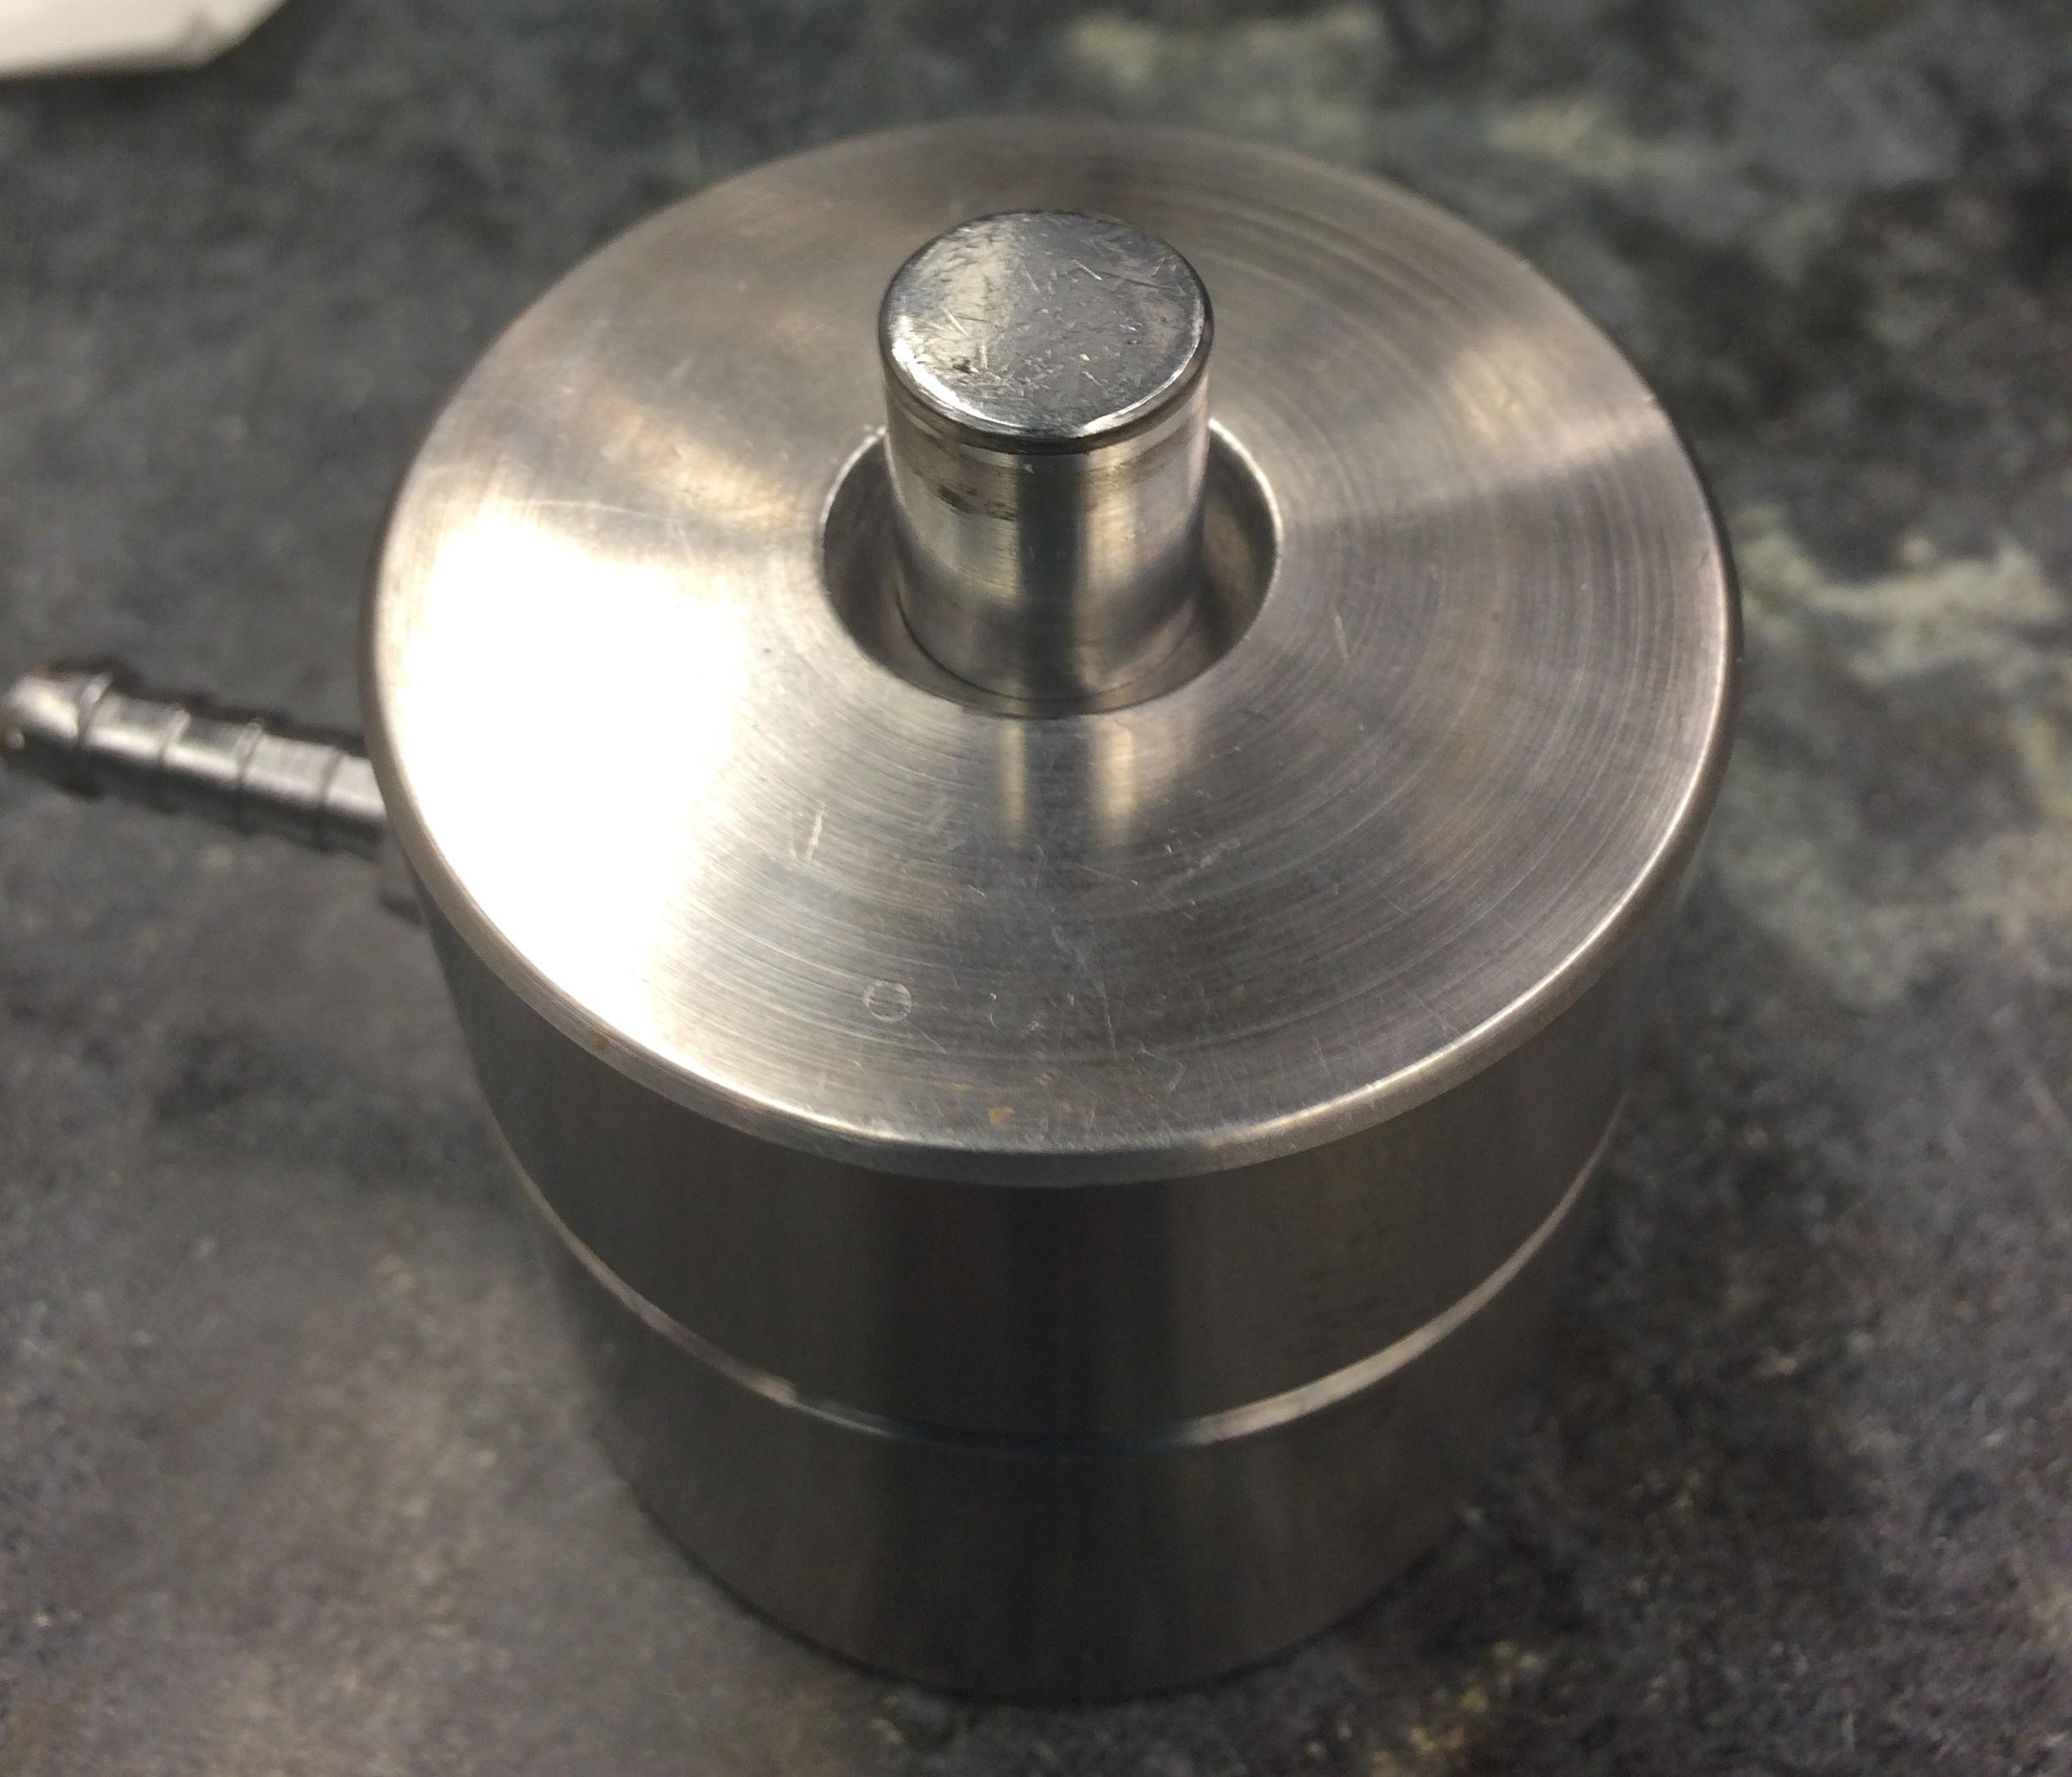
\includegraphics[scale=0.12]{images/die_closed.jpg}
		\caption{Assembled KBr die ready to be compressed.}
		\label{fig:die_closed}
	\end{subfigure}
	\caption{The KBr die used to compress clay powder into pellets.}
	\label{fig:KBr_die}
\end{figure}


Clay which has been pressed into a small thin disk however can be easier to work with in many lab settings, therefore if proper hydration of such samples is possible, they would be of great use in experiments. Such clay disks were prepared for this experiment by placing approximately 0.12$g$ to 0.13$g$ of clay powder into a KBr pellet die. The die used to form the pellets is displayed in Figure~\ref{fig:KBr_die}. A hydraulic press was used to compress the die to a force of approximately 12 tons. A small, sturdy clay pellet or disk was formed with a thickness of approximately 0.5$mm$ and a diameter of 1$cm$. While formed with a KBr die, no KBr was mixed with the clay powder. These samples were then placed in desiccators filled with saturated salt solutions for varying periods of time, until they were removed for XRD measurements. Samples of both types were usually left in desiccators for periods of one to five days before XRD measurements were conducted.

\subsubsection{XRD Measurments}
The $d_{001}$ basal spacing of the samples was measured using a a Bruker D8-Discover X-Ray Diffractometer. Standard locked coupled scans varied the $2\theta$ axis, measuring the reflections at each angle.

Hydrated clay powder was placed into elongated depressions on square glass plates. A second glass plate was then used to press the clay into the depression. After the second plate was removed, large particles of clay on the edge of the depression were wiped away, and the plate was mounted into the diffractometer. A Z scan was first performed to ensure that the X-ray beam was incident in the middle portion of the depression, approximately half way down. Locked coupled scans were performed over the  $2\theta$ angles from $2^\circ$ to $10^\circ$ for all samples.

Hydrated clay pellets underwent a similar process. Pellets were attached to a flat glass plate using a small piece of double sided tape. This plate was then placed in the diffractometer, using 2$mm$ spacer bars to recess the entire plate in the sample mount, to account for the pellet protruding from the surface. A beam height limiter had to be used with the pellets as their diameter was somewhat shorter than most other samples used in the device. A Z scan was again used to center the bean in the center of the disk, between its two faces. A rocking curved scan positioned the $\theta$ axis to the location of maximum intensity, compensating for the fact that the disks do not lie perfectly flat on the plate. Locked coupled scans across the $2\theta$ angle from $2^\circ$ to $10^\circ$ were also performed.

\subsection{Results and Discussion}
\subsubsection{Clay Pellets}

\begin{figure}
	\centering
	\begin{subfigure}{.5\textwidth}
		\centering
		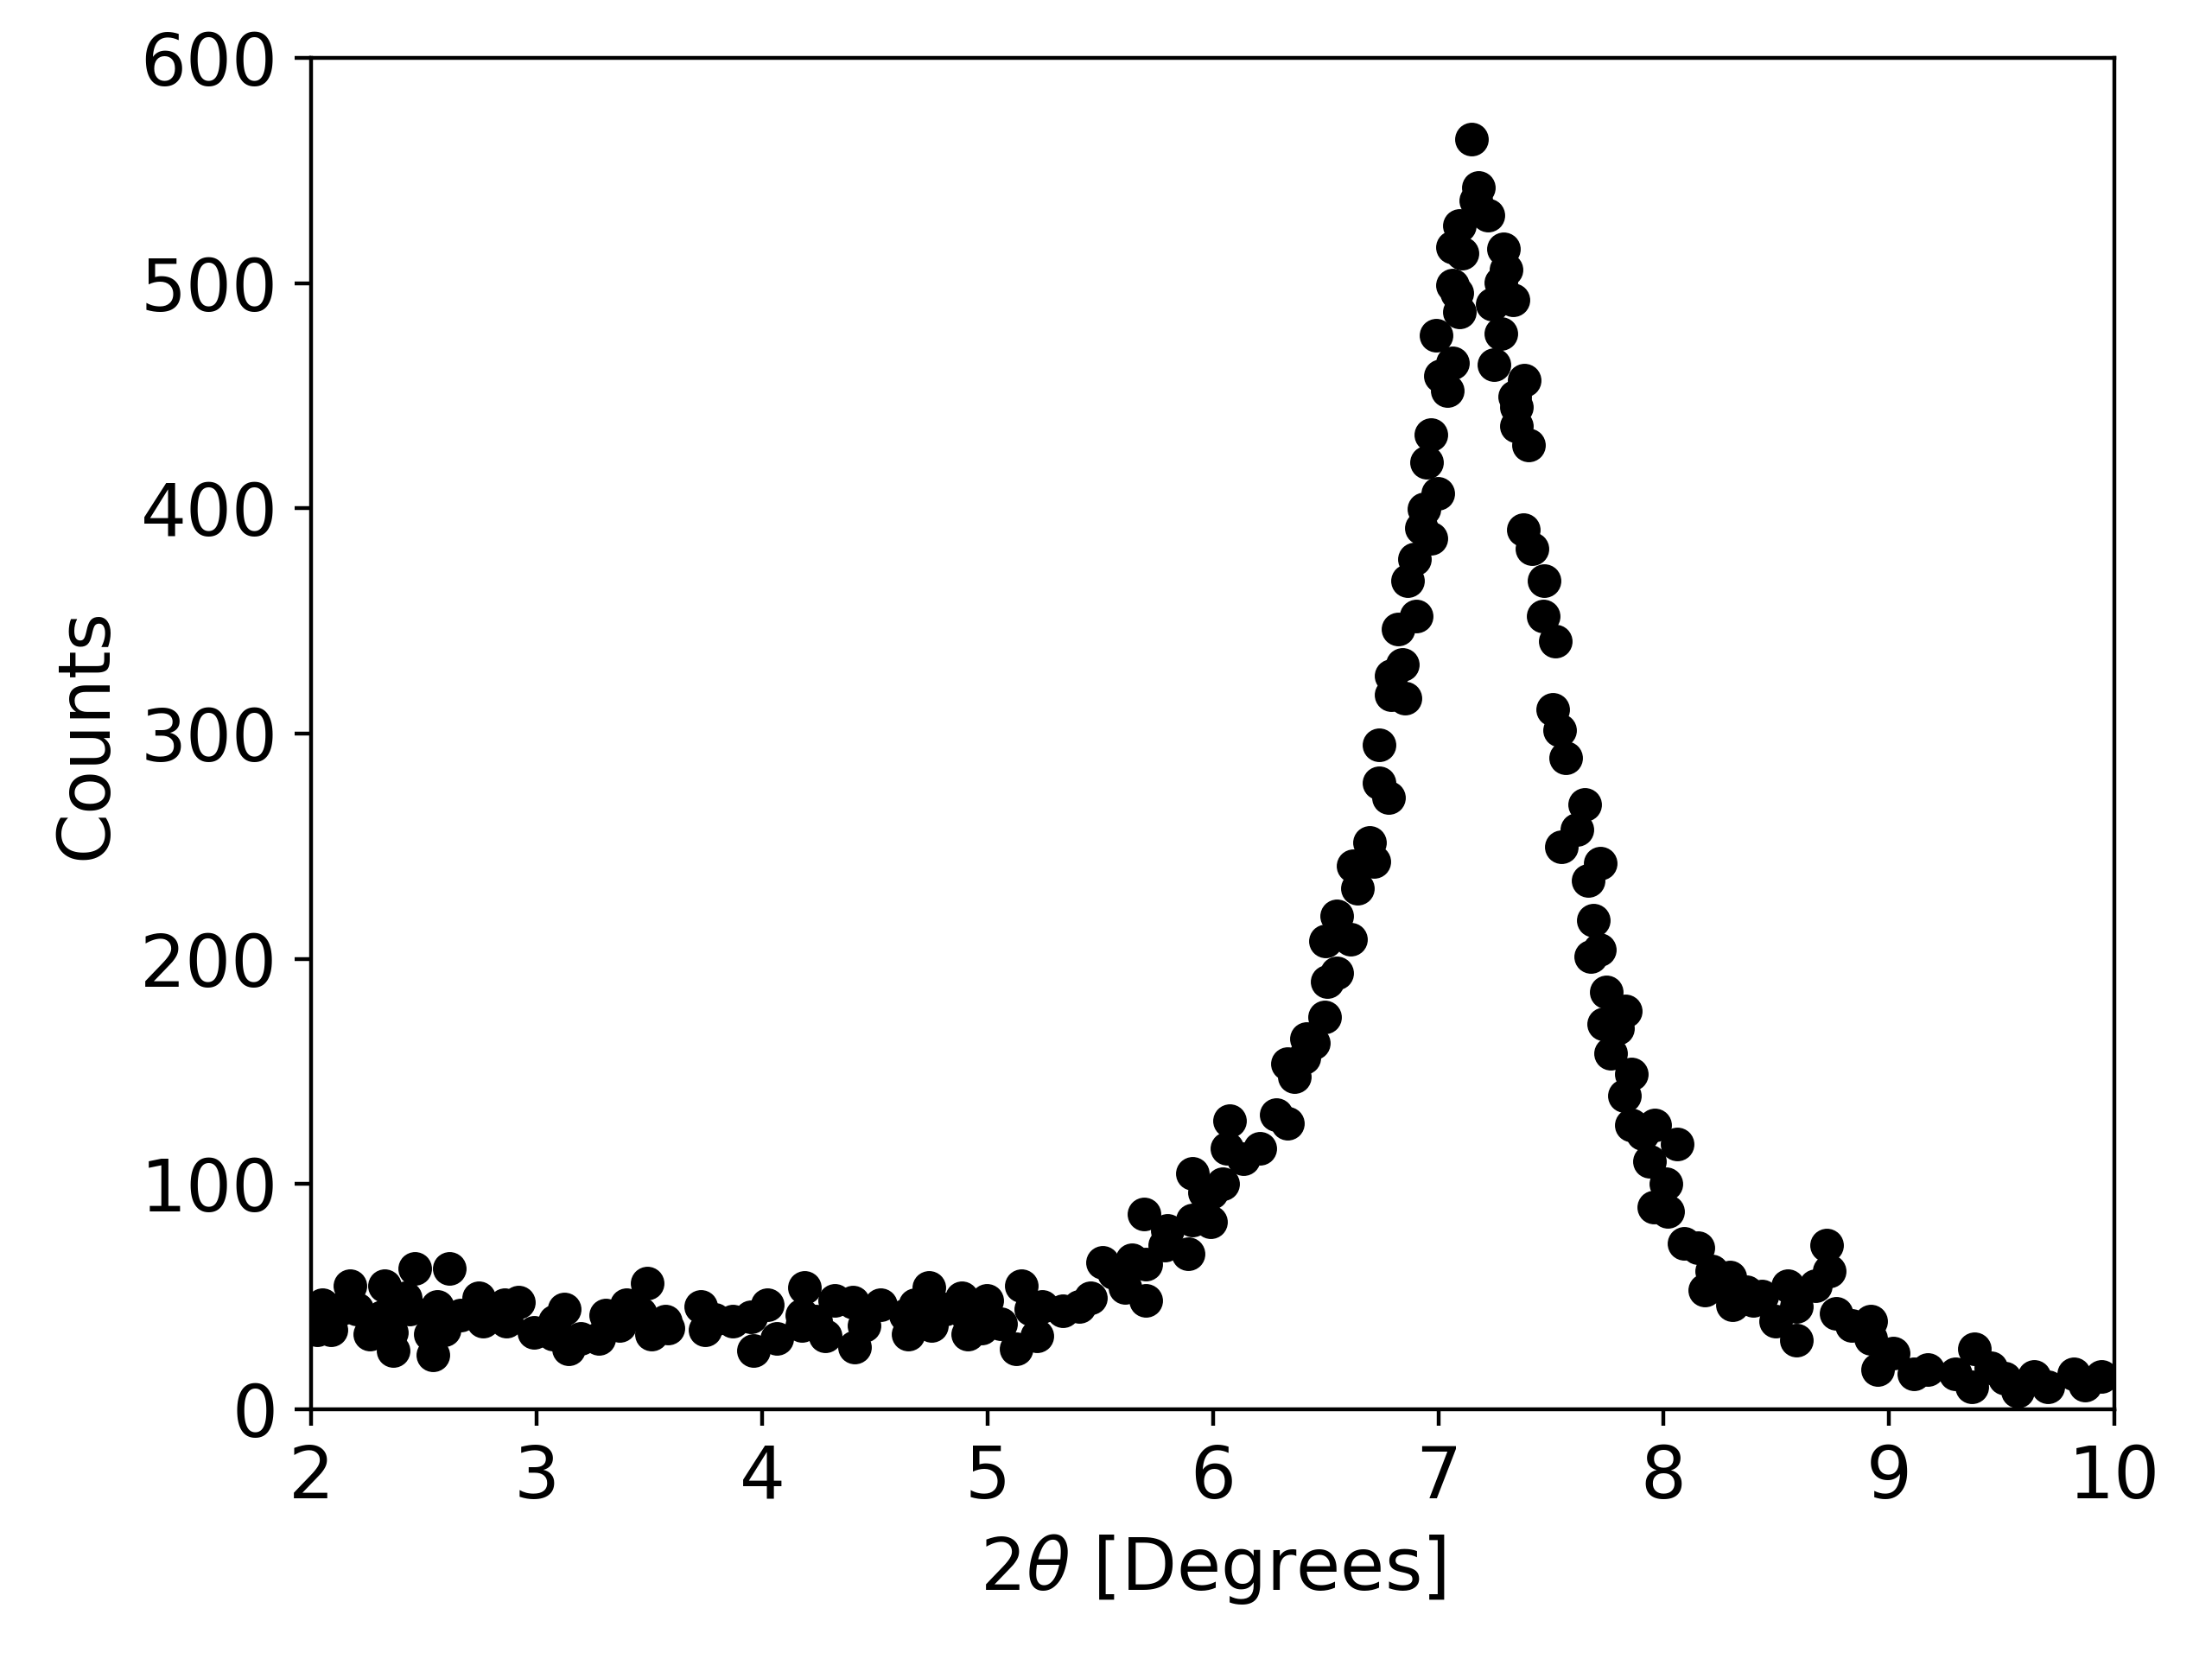
\includegraphics[scale=0.5]{images/80_1d.png}
		\caption{Left for 20 hours, peak at $2\theta=7.1^\circ$ corresponding to $d_{001}=12.4\angstrom$.}
		\label{fig:80_1d}
	\end{subfigure}%
	\begin{subfigure}{.5\textwidth}
		\centering
		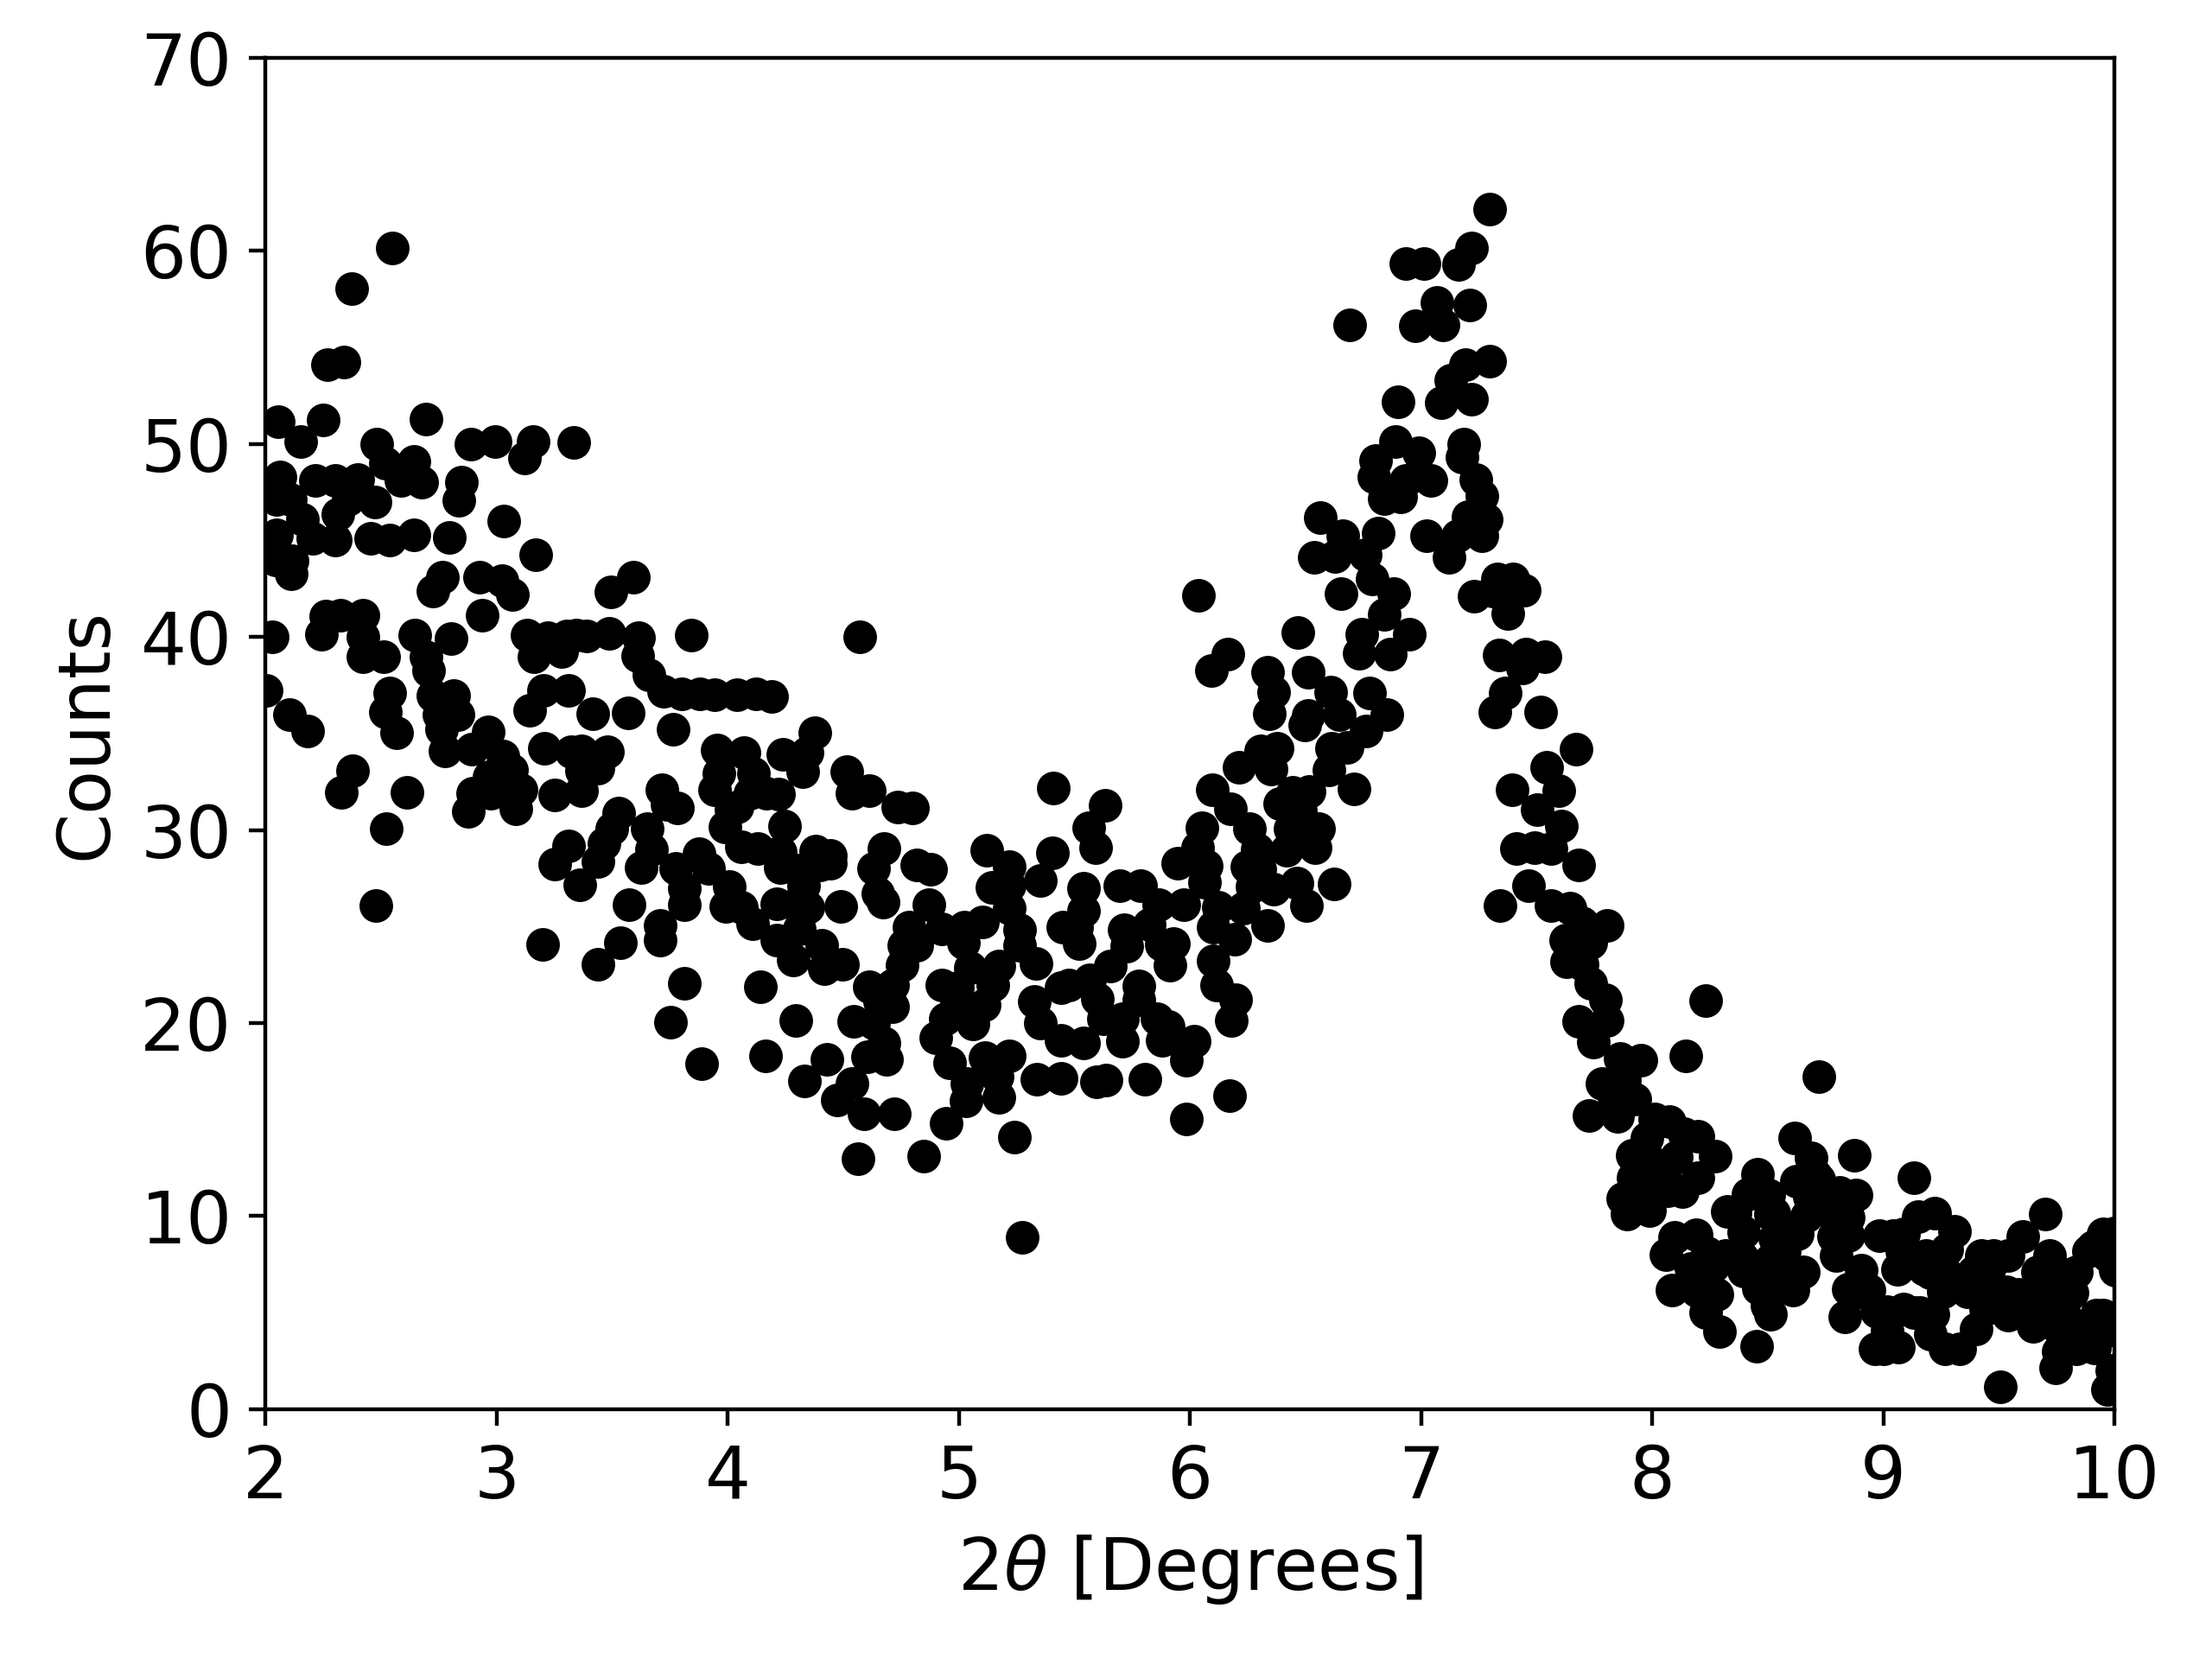
\includegraphics[scale=0.5]{images/80_3d.png}
		\caption{Left for 70 hours, peak at $2\theta=7.3^\circ$ corresponding to $d_{001}=12.1\angstrom$.}
		\label{fig:80_3d}
	\end{subfigure}
	\caption{XRD Bragg peaks of clay pellets left in 80\% humidity.}
	\label{fig:80_pellet}
\end{figure}

The XRD peaks of samples left in desiccators for approximately one and three days are presented in Figure~\ref{fig:80_pellet}. Both peaks indicate that the basal spacing is only $d_{001}\approx 12\angstrom$, indicating that there is only a monolayer of water present in the montmorillonite. The full width half maximum (FWHM) of the peak in Figure~\ref{fig:80_1d} is less than $1^\circ$, indicating that the monolayer is quite homogeneous, and that there are very few, if any locations where there is the formation of a bilayer in the sample. It is more difficult to determine the breadth of the peak in Figure~\ref{fig:80_3d}, but due to the smaller basal spacing in accordance with the center of the peak location, it is also very likely that there is but a monolayer of water present between the clay sheets.

\begin{figure}
	\centering
	\begin{subfigure}{.5\textwidth}
		\centering
		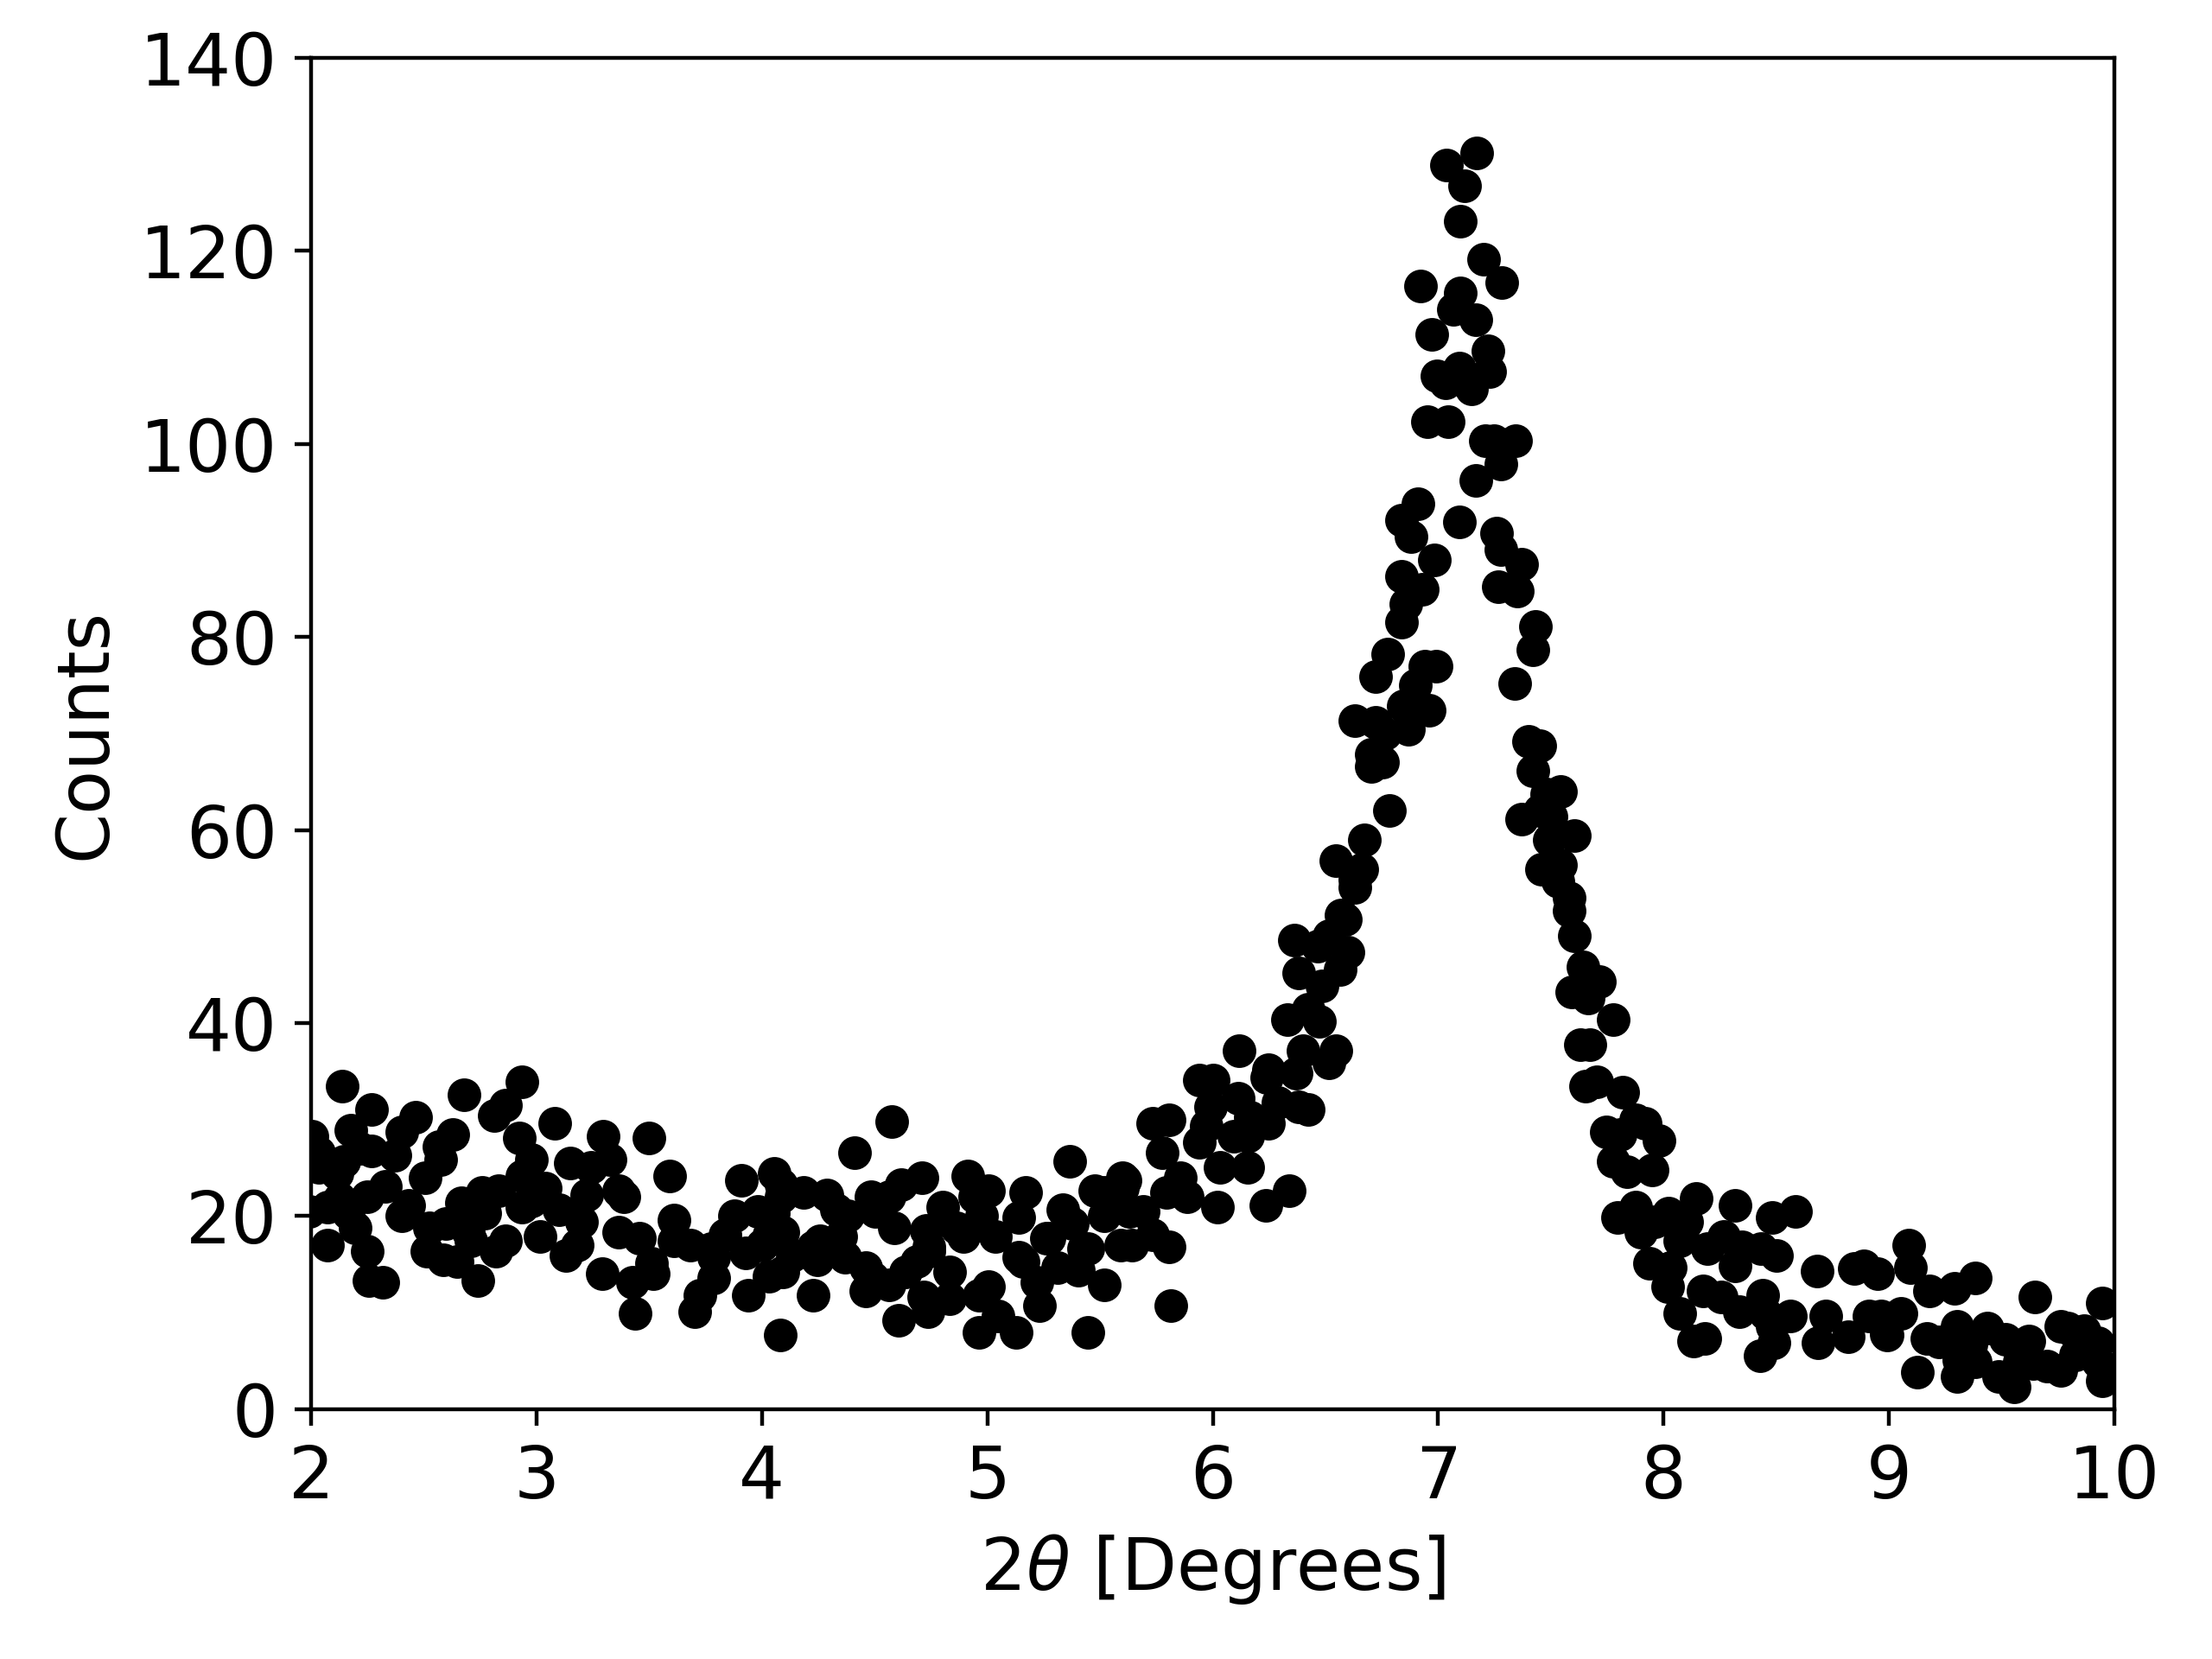
\includegraphics[scale=0.5]{images/97_plt_1d.png}
		\caption{Left for 20 hours, peak at $2\theta=7.2^\circ$ corresponding to $d_{001}=12.3\angstrom$.}
		\label{fig:97_plt_1d}
	\end{subfigure}%
	\begin{subfigure}{.5\textwidth}
		\centering
		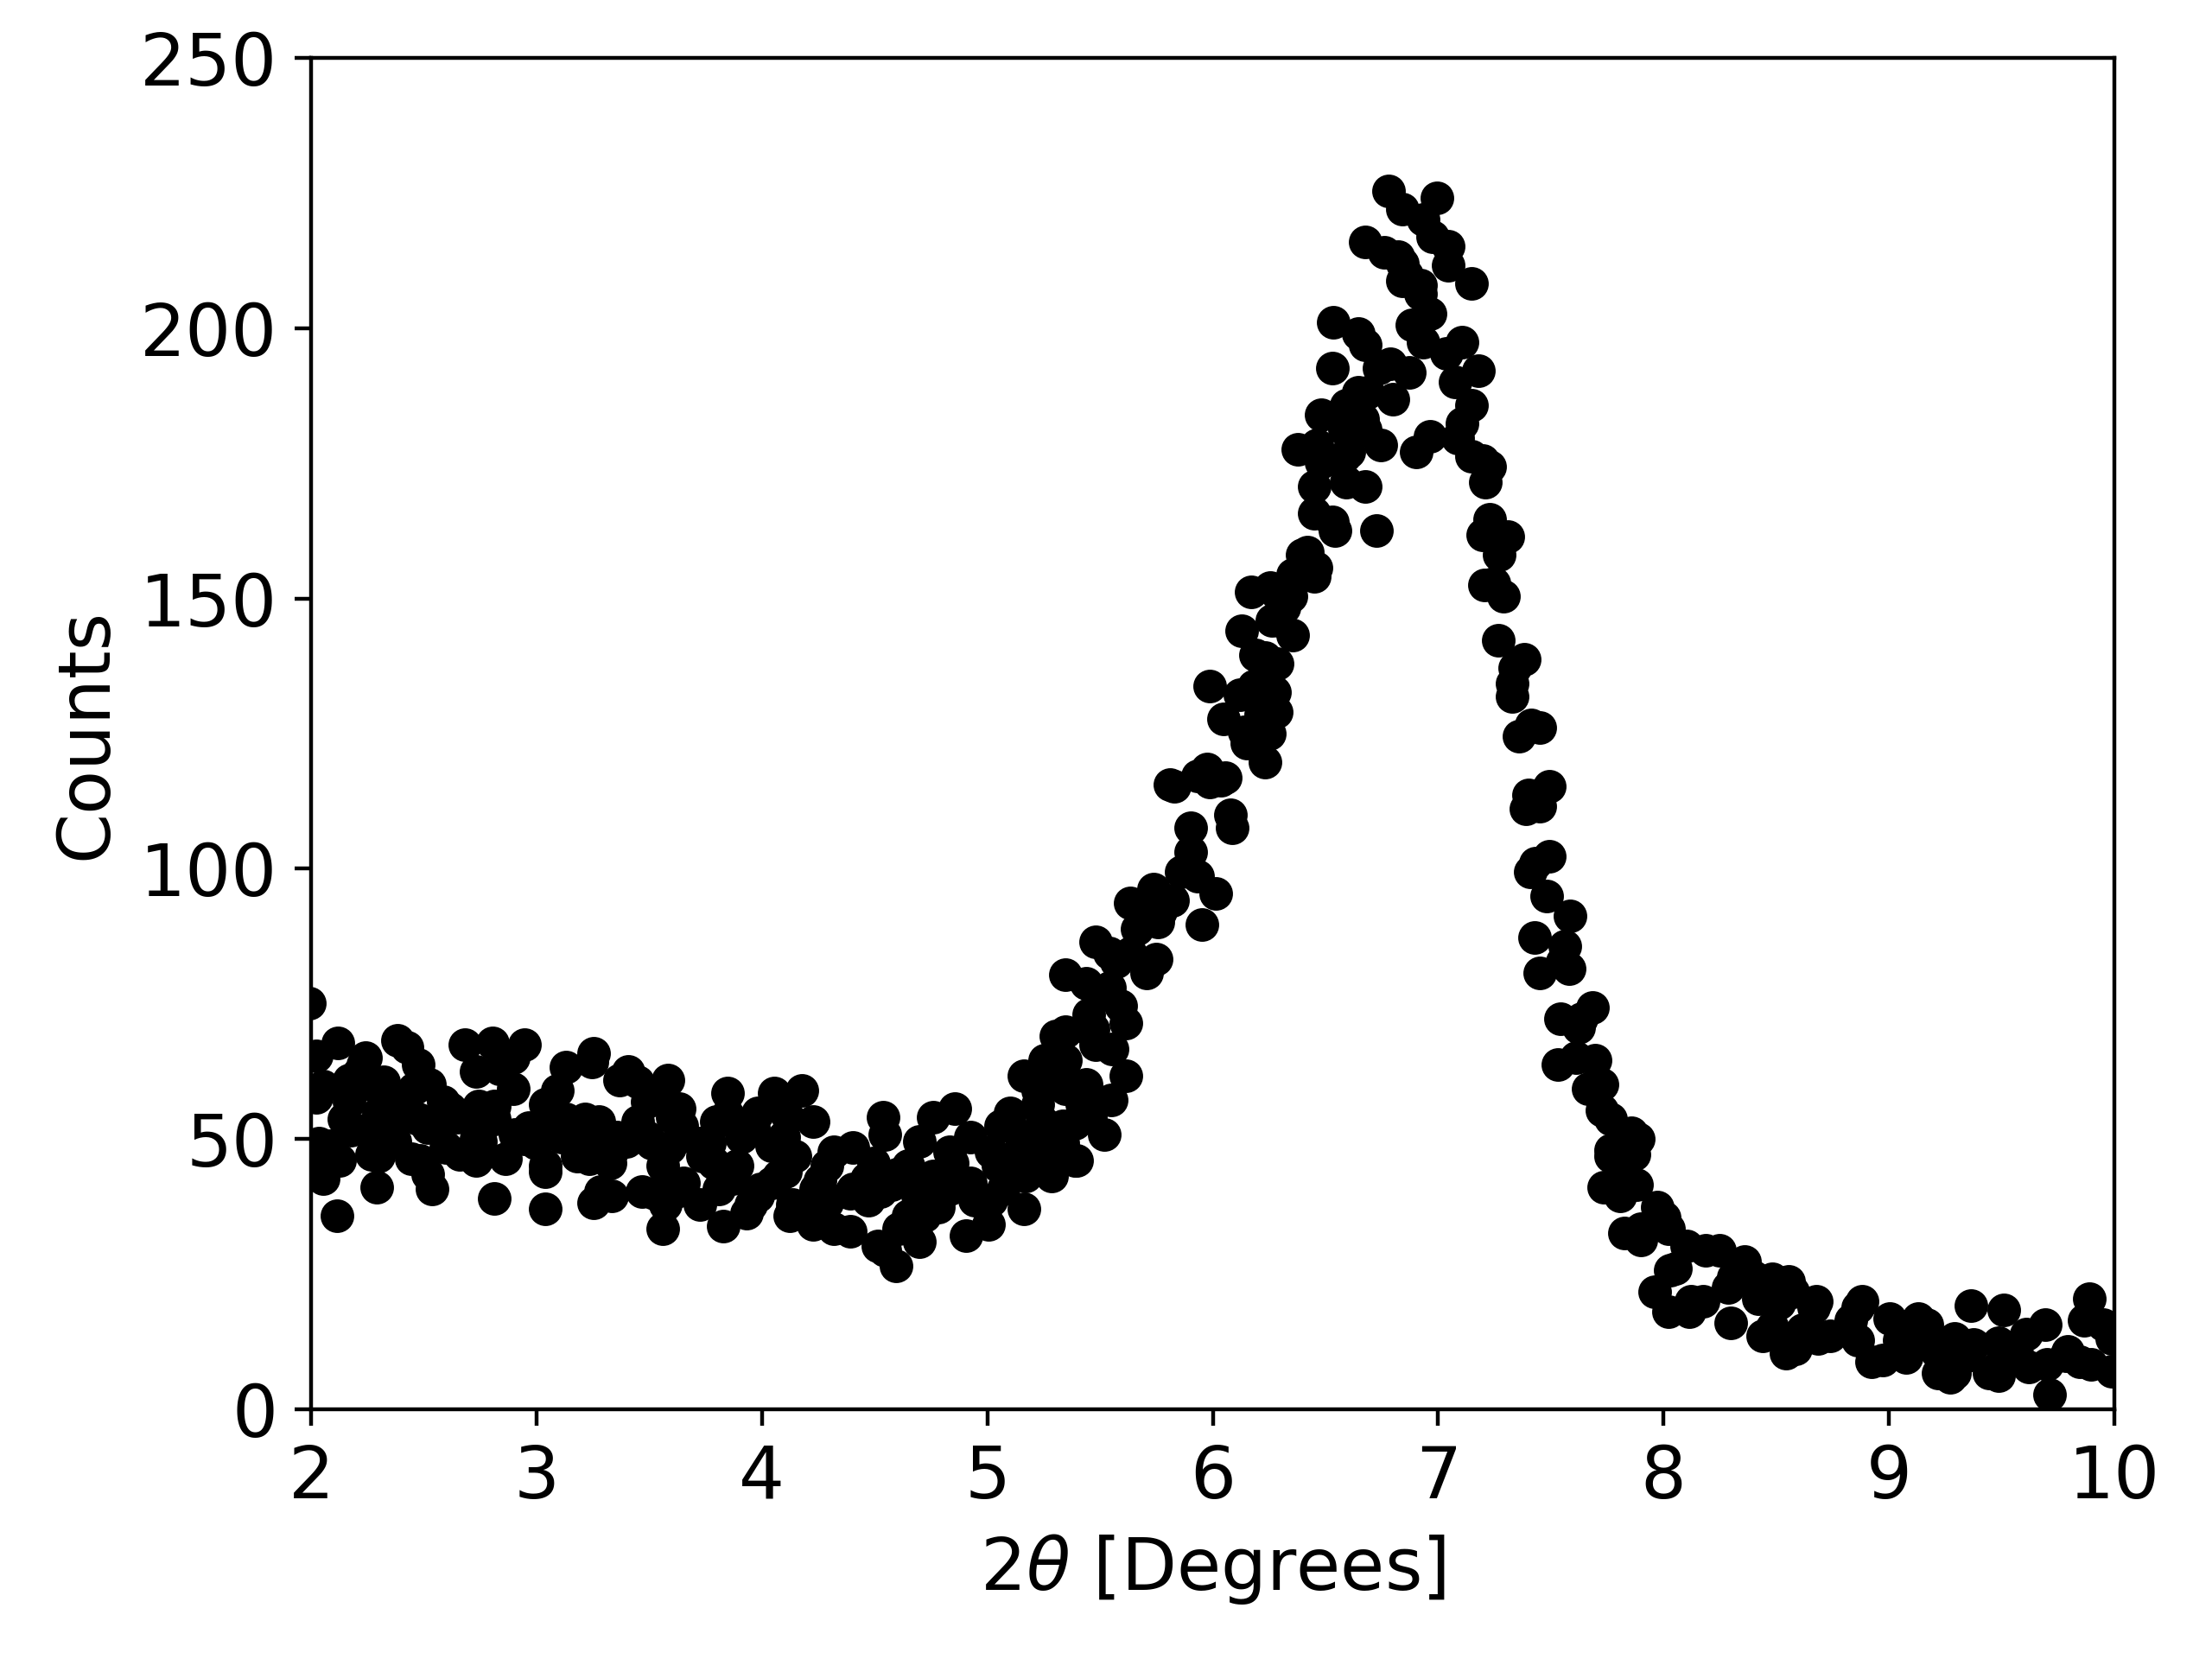
\includegraphics[scale=0.5]{images/97_plt_3d.png}
		\caption{Left for 70 hours, peak at $2\theta=7.0^\circ$ corresponding to $d_{001}=12.7\angstrom$.}
		\label{fig:97_plt_3d}
	\end{subfigure}
	\caption{XRD Bragg peaks of clay pellets left in 97\% humidity.}
	\label{fig:97_pellet}
\end{figure}

Moving up in humidity to the $K_2SO_4$ desiccator, which should have maintained a relative humidity of $p/p_0=0.97$, a similar result is observed. After one day, as shown in Figure~\ref{fig:97_plt_1d}, the sample only has a monolayer of water which is very homogeneous. Increasing the time it is left in the desiccator to three days does have a slight effect. As seen in Figure~\ref{fig:97_plt_3d}, the main peak is still at $7.3^\circ$, indicating a monolayer, but a small bump is now visible at approximately $5.5^\circ$, which corresponds to a bilayer of water. Although small, this does indicate a certain level of heterogeneity in the hydration.


\subsubsection{Clay Powder}

\begin{figure}
	\centering
	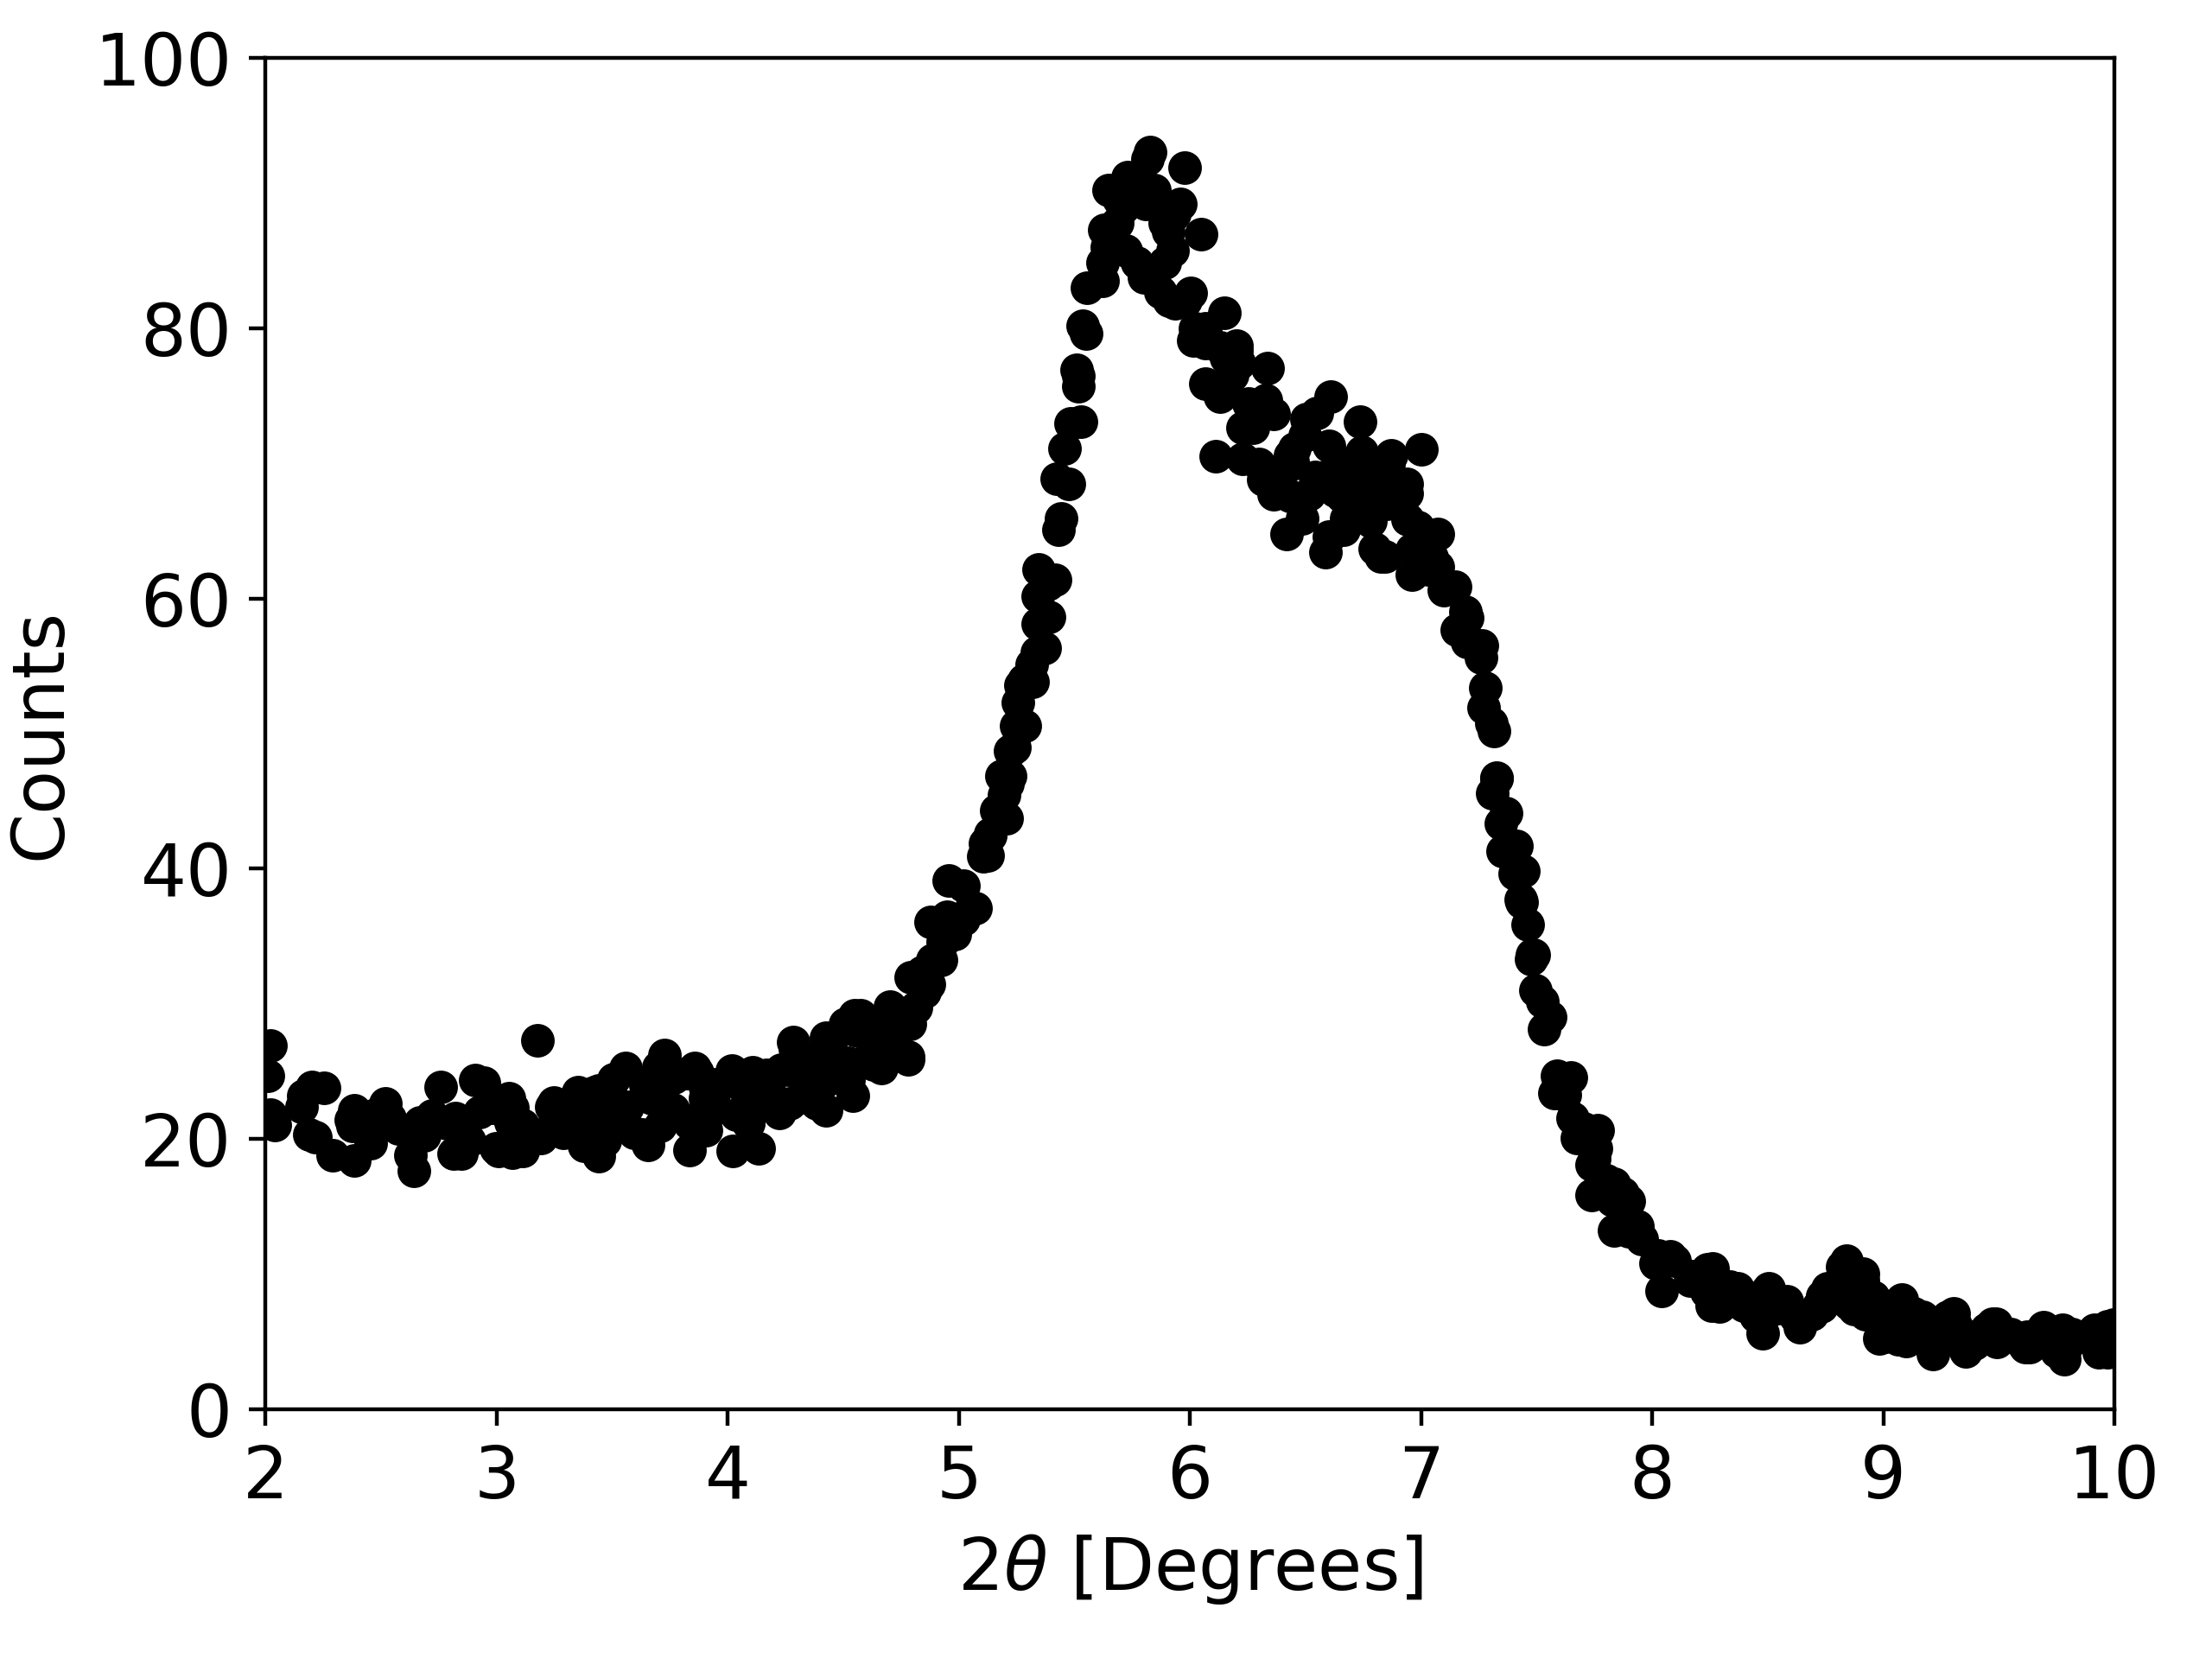
\includegraphics[scale=0.7]{images/97_pwd_3d.png}
	\caption{Peak of clay powder kept at 97\% humidity for three days, with $d_{001}=15.1\angstrom$, and a FWHM of $2.0^\circ$.}
	\label{fig:97_pwd_3d}
\end{figure}

Leaving clay powder samples at 97\% humidity for three days produces a very different result compared to the clay pellets which were exposed for a comparable amount of time. In Figure~\ref{fig:97_pwd_3d}, we see that the principal peak is now that corresponding to a $15.1\angstrom$ basal spacing, indicating a bilayer of water, and a second peak, of just a slightly lower magnitude, is observed at $2\theta=7^\circ$, corresponding to a monolayer of water. From this, it would appear that the powder samples are much more easily hydrated than the clay pellets, and that in this sample, there is mainly a bilayer of water between sheets of clay, though it is very heterogeneous, with a large portion of the clay also having a monolayer.

\begin{figure}
	\centering
	\begin{subfigure}{.5\textwidth}
		\centering
		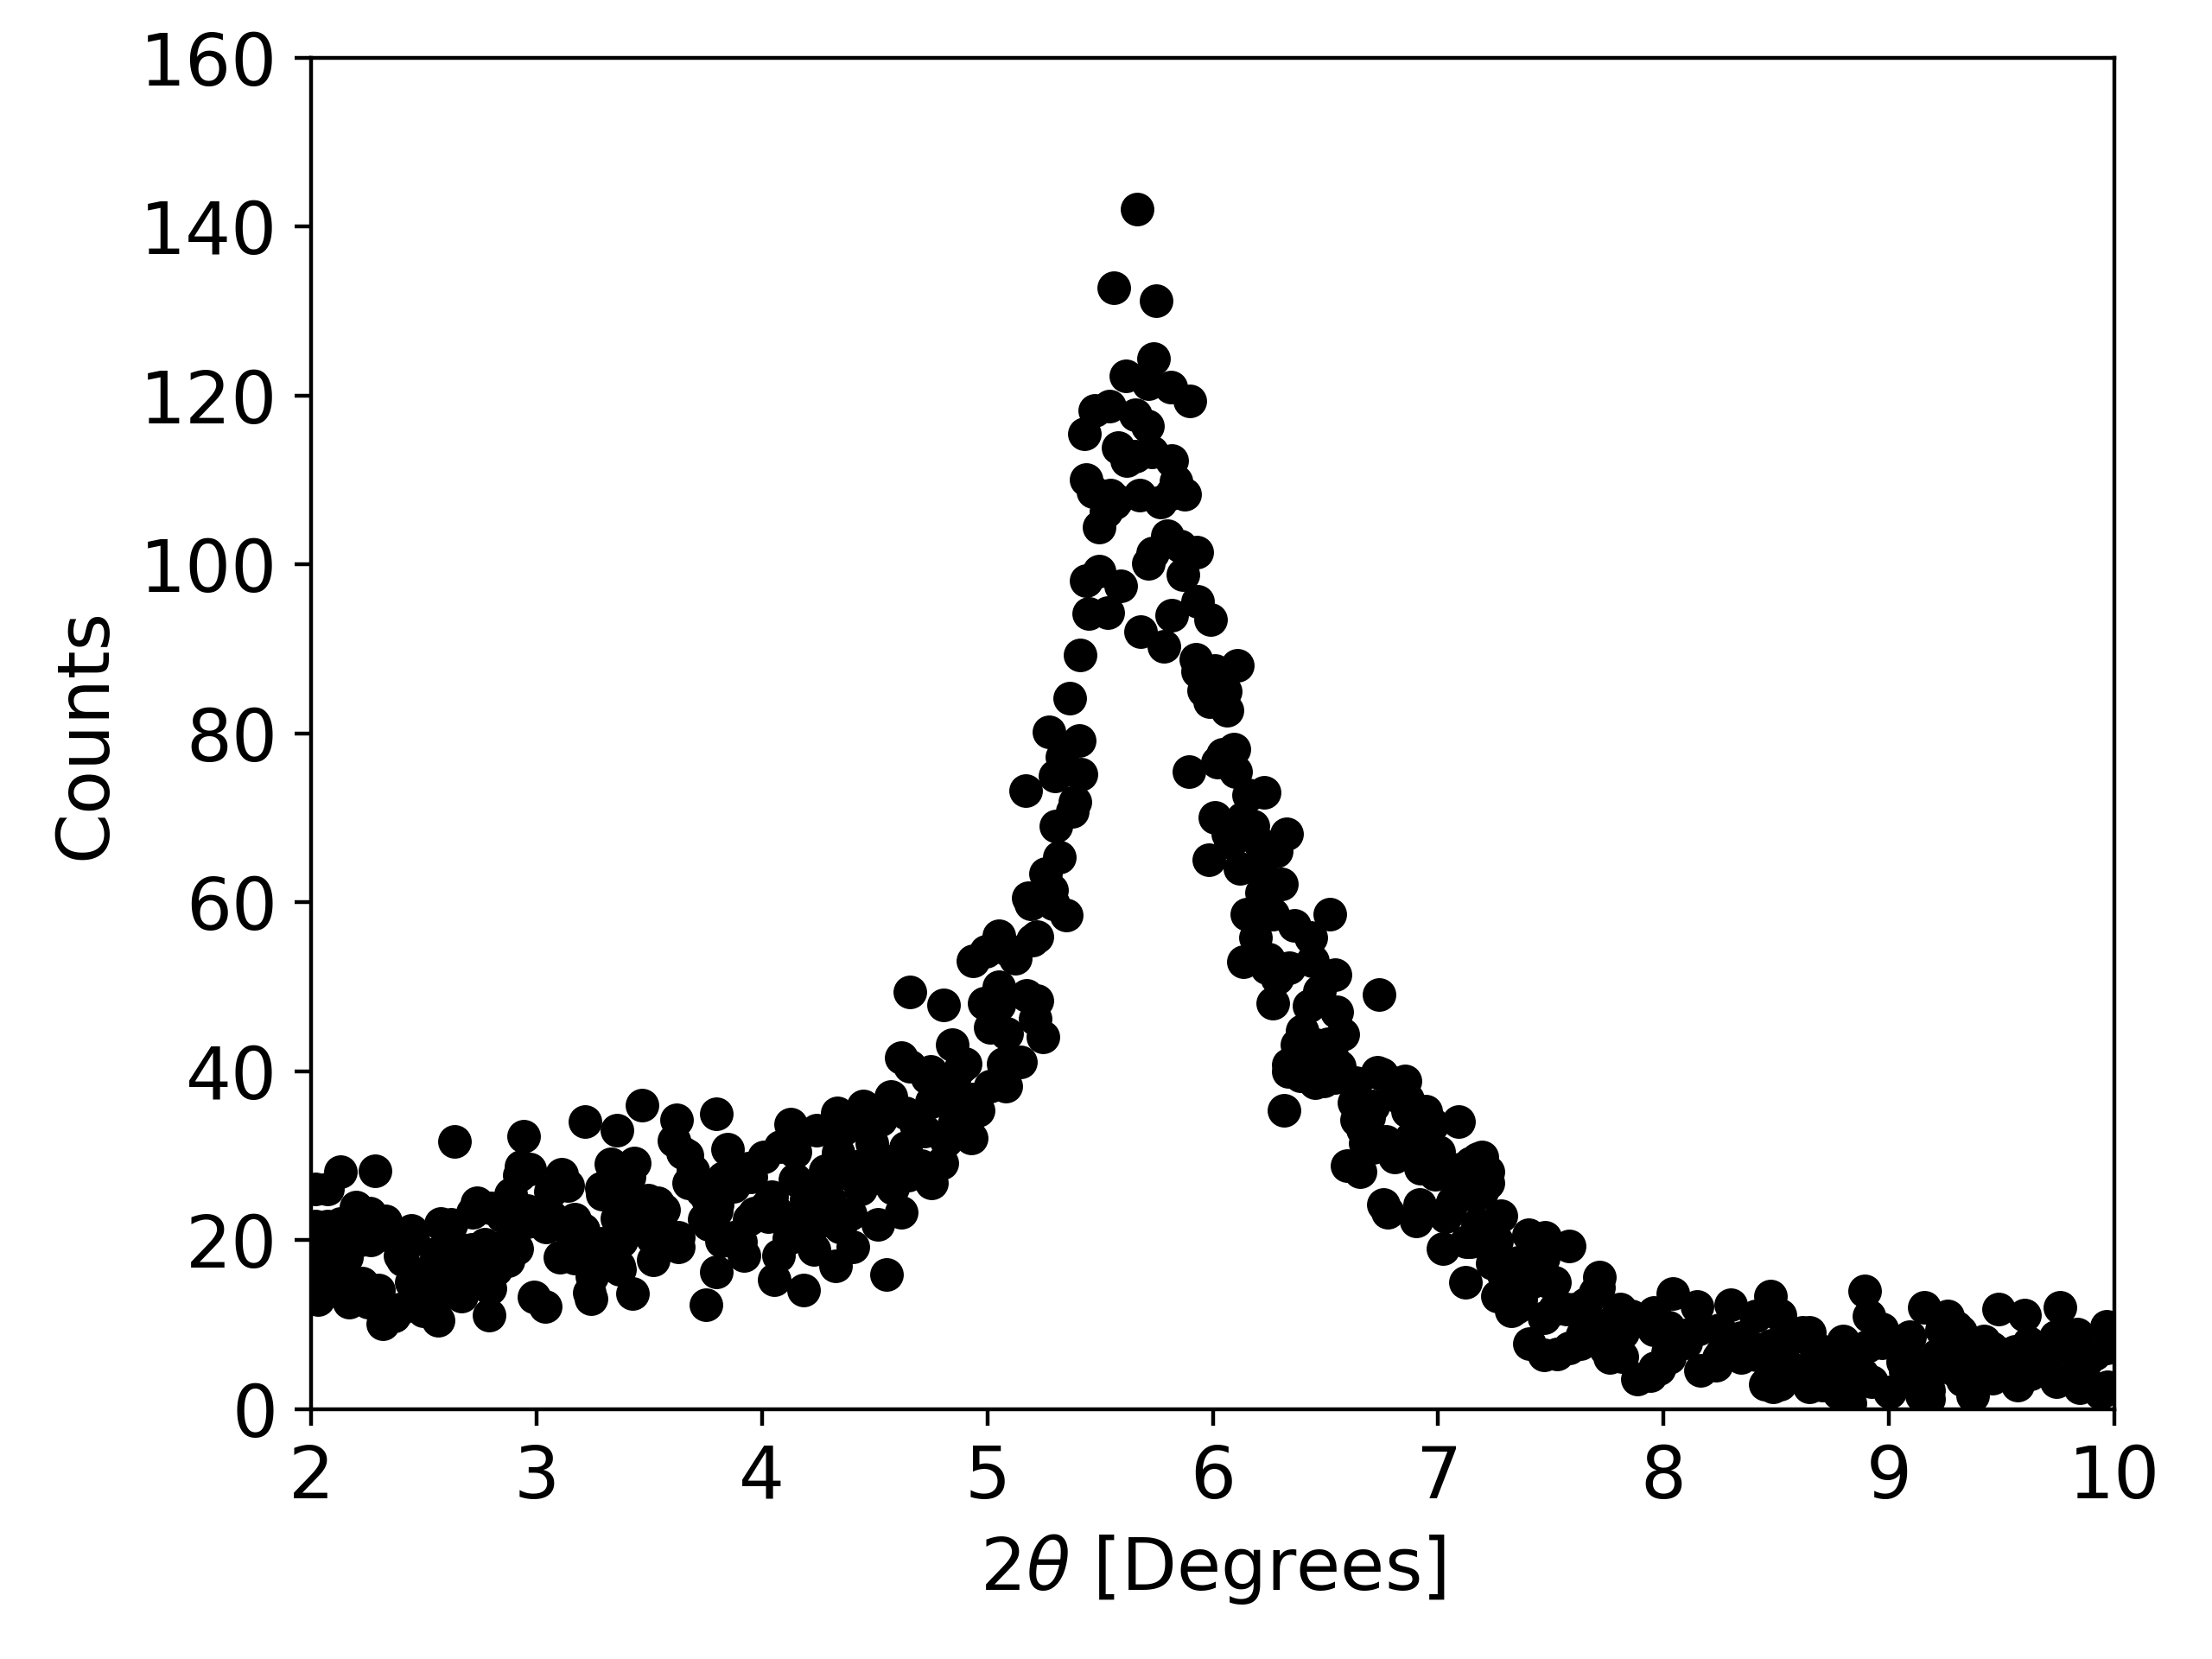
\includegraphics[scale=0.5]{images/97_pwd_5d.png}
		\caption{Initial scan, basal spacing of $d_{001}=15.5\angstrom$ and FWHM of $0.8^\circ$.}
		\label{fig:97_pwd_5d}
	\end{subfigure}%
	\begin{subfigure}{.5\textwidth}
		\centering
		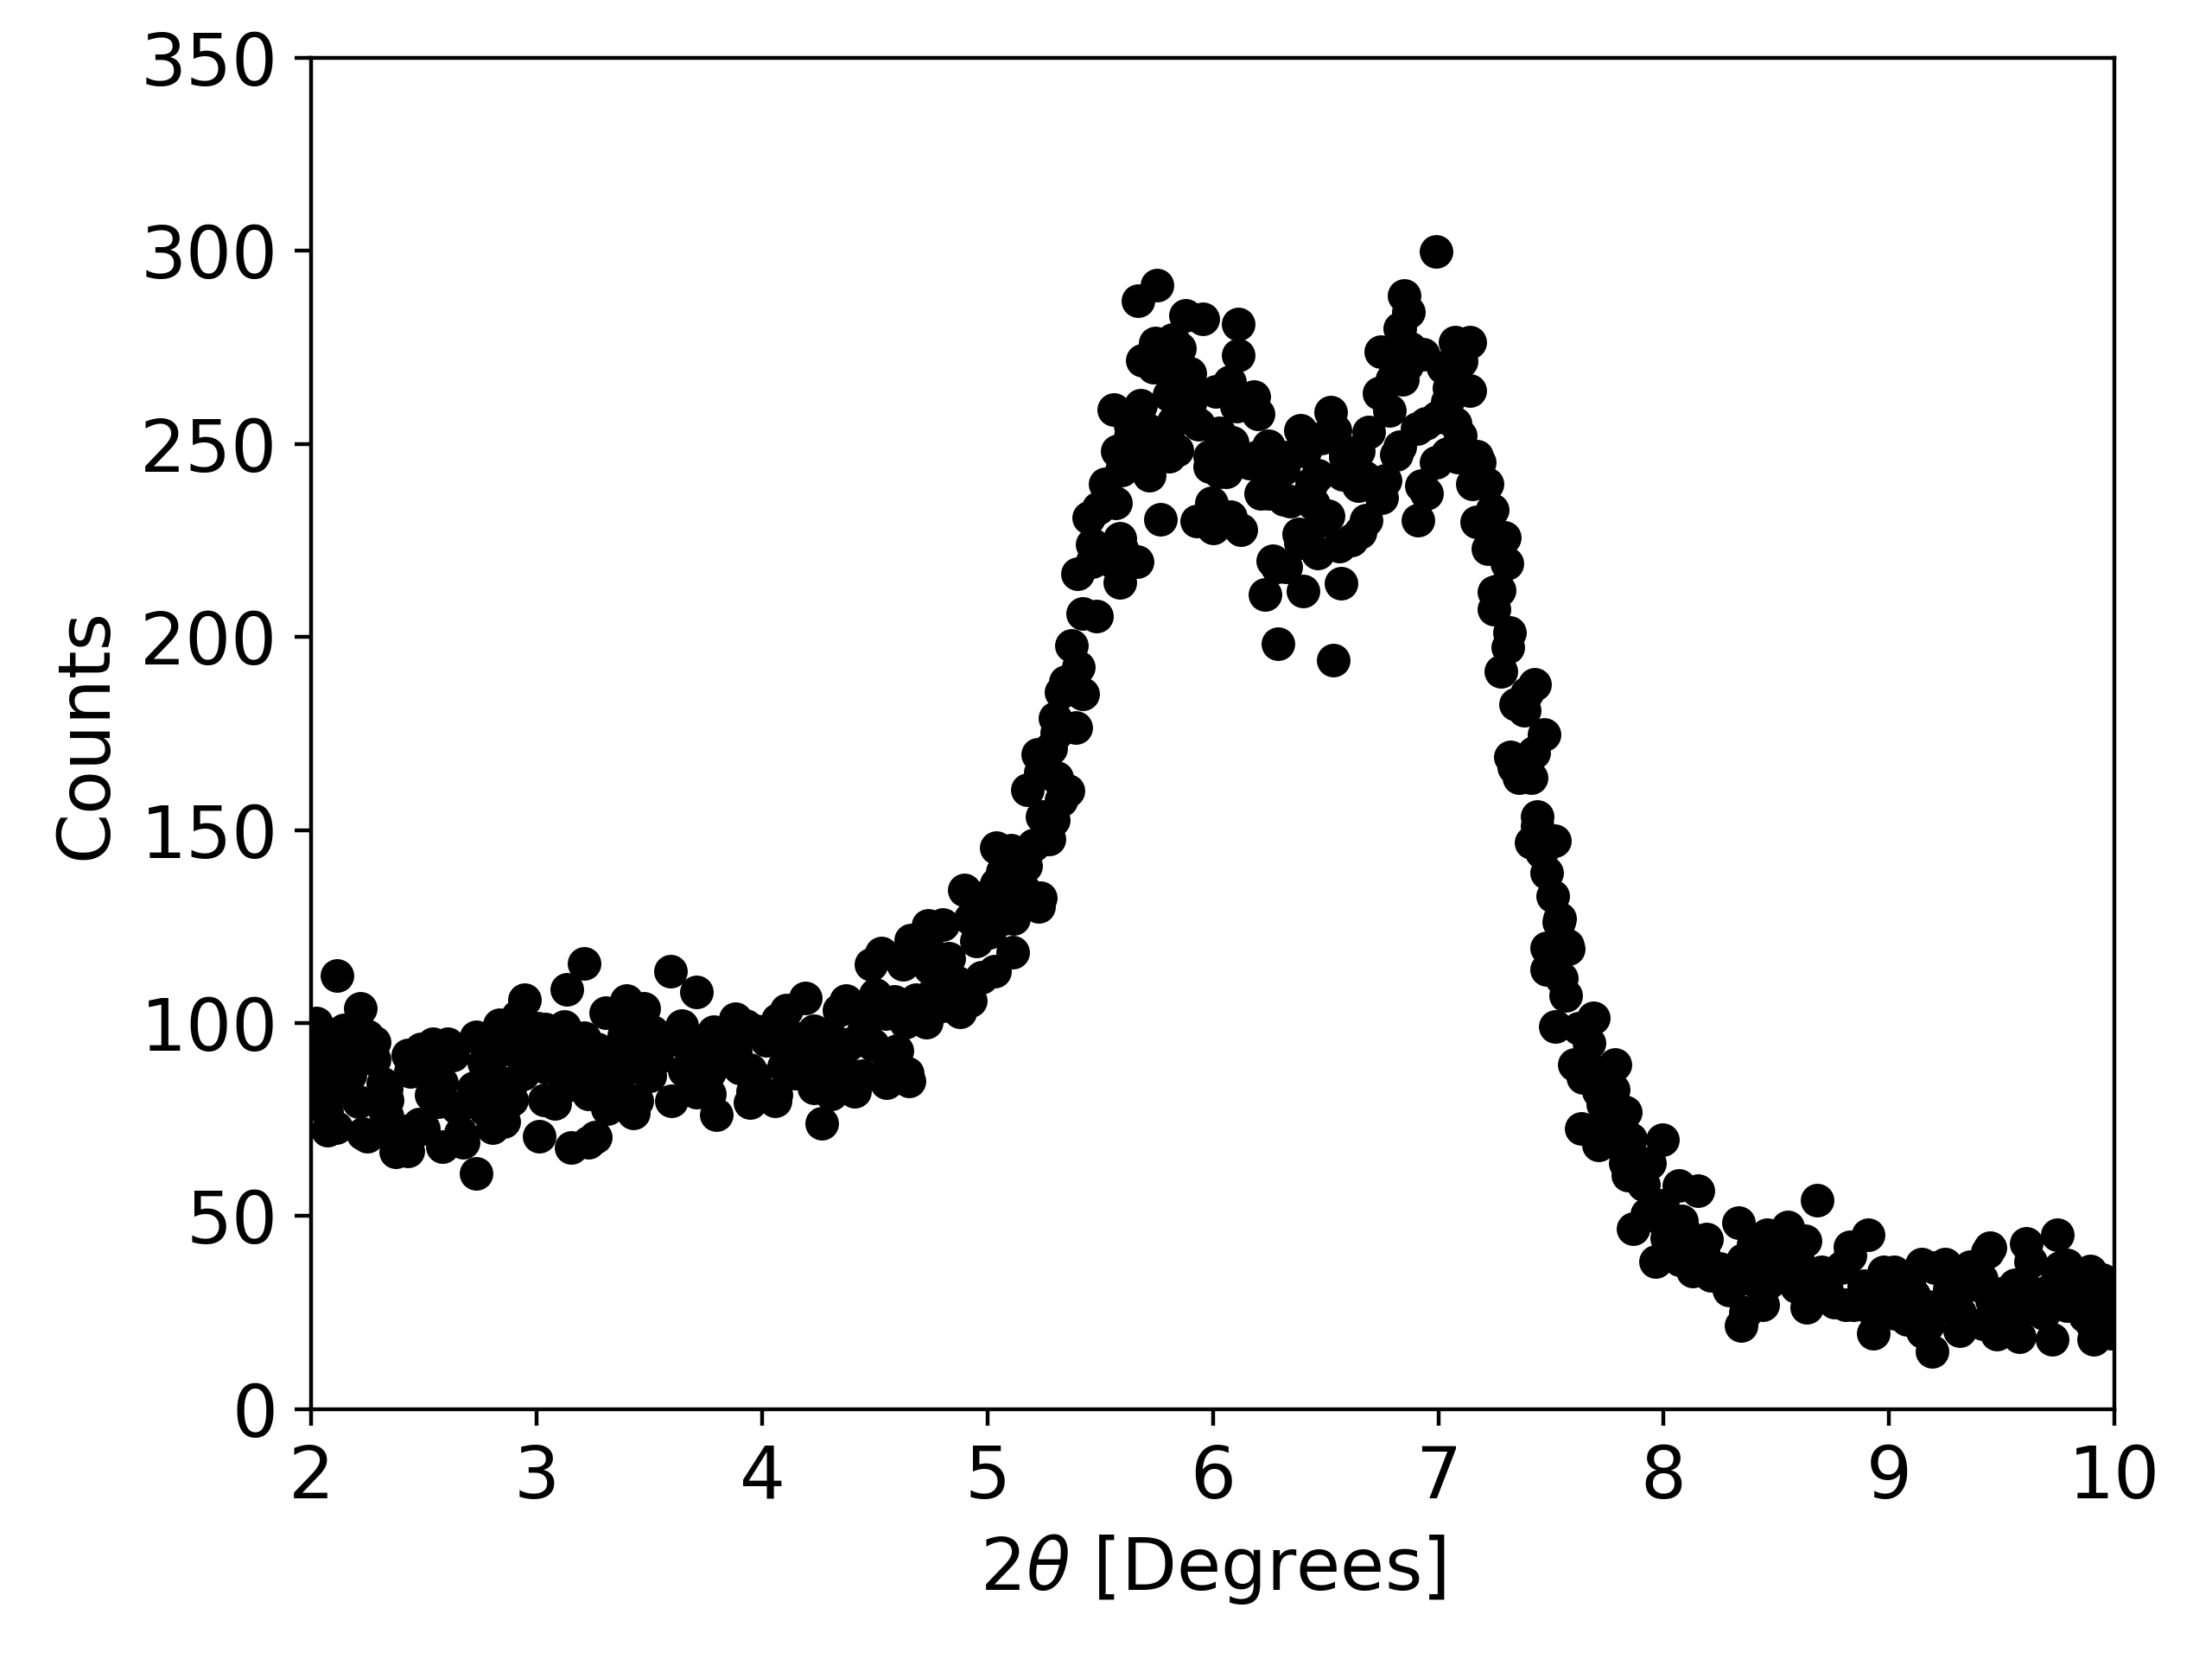
\includegraphics[scale=0.5]{images/97_pwd_5d_2.png}
		\caption{Second scan taken 15 minutes later. Peaks for spacing of $15.5\angstrom$ and $12.5\angstrom$.}
		\label{fig:97_pwd_5d_2}
	\end{subfigure}
	\caption{Bragg peaks of clay powder left in 97\% humidity for five days.}
	\label{fig:97_pwd_double}
\end{figure}

Upon increasing the duration for which the clay powder was left in the desiccator at 97\% humidity to five days, it was initially found that the sample had a near homogeneous bilayer of water intercalated between clay sheets. This peak may be observed in Figure~\ref{fig:97_pwd_5d}. There is a very small peak present at $7^\circ$, indicating some portions of the sample with only a monolayer, but the FWHM of the principal peak being less than $1^\circ$ indicated a very homogeneous bilayer hydration. While performing the scan however, which could take upwards of 20 minutes per sample, it was observed that the signal was changing with time. In Figure~\ref{fig:97_pwd_5d_2}, the signal of the exact same sample, but scanned 15 minutes later is presented. There is a very clear double peak, indicating that the sample now roughly has a 50\% bilayer and 50\% monolayer hydration. Observing this shift has shown just how sensitive the clay samples are to changes in the ambient relative humidity, and that while it may take the clay several days to obtain a homogeneous bilayer hydrate, this water may be lost in a matter of minutes if there is a large decrease in ambient humidity. Unfortunately, there is no way of knowing what the humidity in the XRD chamber was while these measurements were taken.

\subsubsection{Overview}
From this experiment, it is evident that the hydration of clay powder samples is much easier than that of the compressed clay pellets. This is likely due to the decreased surface area of clay which is in contact with the air for the clay pellets in comparison to the powder. It is also likely more difficult for the pellets to swell and expand due to their being too firmly compressed. More experiments would have to be conducted for longer periods of time to determine whether or not it is even possible to achieve a homogeneous bilayer hydration of a clay pellet. Such a task is manageable however if the clay is left in powder form, though the times required are much higher than those reported by Bérend et. al. \cite{berend1995mechanism}. Table~\ref{tab:hyd_time} provides a summary of the required times for different hydration levels. One reason for the greater times reported here is that the humidity inside of the desiccators might not have been that predicted by the prescribed salt solution. It is possible that the plastic desiccators used were not very airtight, or that there was not enough salt solution in each desiccator. Actually measuring the relative humidity is quite difficult, and requires expensive equipment which was not available. As such, all of the reported humidities in this work must be considered rough estimates at best. Despite this fact, these results should be easily reproducible with the specified salt solutions, and may even provide higher hydration levels in shorter periods of time if more salt solution or better desiccators are used.
\begin{table}
	\centering
	\caption{Times and humidities required for various hydration levels of Li montmorillonite.}
	\label{tab:hyd_time}
	\begin{tabular}{|c|c|c|c|}
		\hline
		\textbf{Humidity [$\bm{p/p_0}$]} & \textbf{Sample Type} & \textbf{Time [$\bm{hr}$]} & \textbf{Hydration} \\
		\hline
		\hline
		0.8 & pellet & 70 & monolayer \\
		\hline
		0.97 & pellet & 70 & monolayer, some bilayer \\
		\hline
		0.97 & powder & 70 & bilayer, large portion monolayer \\
		\hline
		0.97 & powder & 120 & bilayer \\
		\hline		
	\end{tabular}
\end{table}


%%% Local Variables: 
%%% mode: latex
%%% TeX-master: t
%%% End: 
